%%%%%%%%%%%%%%%%%%%%%%%%%%%%%%%%%%%%%%%%%
% Journal Article
% LaTeX Template
% Version 1.4 (15/5/16)
%
% This template has been downloaded from:
% http://www.LaTeXTemplates.com
%
% Original author:
% Frits Wenneker (http://www.howtotex.com) with extensive modifications by
% Vel (vel@LaTeXTemplates.com)
%
% License:
% CC BY-NC-SA 3.0 (http://creativecommons.org/licenses/by-nc-sa/3.0/)
%
%%%%%%%%%%%%%%%%%%%%%%%%%%%%%%%%%%%%%%%%%

%----------------------------------------------------------------------------------------
%	PACKAGES AND OTHER DOCUMENT CONFIGURATIONS
%----------------------------------------------------------------------------------------

\documentclass[twoside,onecolumn]{article}

\usepackage{blindtext} % Package to generate dummy text throughout this template 

\usepackage[sc]{mathpazo} % Use the Palatino font
\usepackage[T1]{fontenc} % Use 8-bit encoding that has 256 glyphs
\linespread{1.05} % Line spacing - Palatino needs more space between lines
\usepackage{microtype} % Slightly tweak font spacing for aesthetics

\usepackage[english]{babel} % Language hyphenation and typographical rules

\usepackage[hmarginratio=1:1,top=32mm,columnsep=20pt]{geometry} % Document margins
\usepackage[hang, small,labelfont=bf,up,textfont=it,up]{caption} % Custom captions under/above floats in tables or figures
\usepackage{booktabs} % Horizontal rules in tables

\usepackage{lettrine} % The lettrine is the first enlarged letter at the beginning of the text

\usepackage{enumitem} % Customized lists
\setlist[itemize]{noitemsep} % Make itemize lists more compact

\usepackage{abstract} % Allows abstract customization
\renewcommand{\abstractnamefont}{\normalfont\bfseries} % Set the "Abstract" text to bold
\renewcommand{\abstracttextfont}{\normalfont\small\itshape} % Set the abstract itself to small italic text

\usepackage{titlesec} % Allows customization of titles
\renewcommand\thesection{\Roman{section}} % Roman numerals for the sections
\renewcommand\thesubsection{\roman{subsection}} % roman numerals for subsections
\titleformat{\section}[block]{\large\scshape\centering}{\thesection.}{1em}{} % Change the look of the section titles
\titleformat{\subsection}[block]{\large}{\thesubsection.}{1em}{} % Change the look of the section titles

\usepackage{fancyhdr} % Headers and footers
\pagestyle{fancy} % All pages have headers and footers
\fancyhead{} % Blank out the default header
\fancyfoot{} % Blank out the default footer
\fancyhead[C]{Harvey Hughes $\bullet$ March 2019 $\bullet$ Emmanuel College} % Custom header text
\fancyfoot[RO,LE]{\thepage} % Custom footer text

\usepackage{titling} % Customizing the title section

\usepackage{hyperref} % For hyperlinks in the PDF

\usepackage{graphicx}
\graphicspath{ {images/} }

\newenvironment{reusefigure}[2][htbp]
  {\addtocounter{figure}{-1}%
   \renewcommand{\theHfigure}{dupe-fig}% If you're using hyperref
   \renewcommand{\thefigure}{\ref{#2}}% Figure counter is \ref
   \renewcommand{\addcontentsline}[3]{}% Avoid placing figure in LoF
   \begin{figure}[#1]}
  {\end{figure}}
\usepackage{wrapfig}
\usepackage{amsmath}
\usepackage{xcolor}
\usepackage{listings}
\usepackage{subcaption}
\usepackage{pdfpages}

%----------------------------------------------------------------------------------------
%	TITLE SECTION
%----------------------------------------------------------------------------------------

\setlength{\droptitle}{-4\baselineskip} % Move the title up

\pretitle{\begin{center}\Huge\bfseries} % Article title formatting
\posttitle{\end{center}} % Article title closing formatting
\title{3C6 Digital Vibration Analysis FTR} % Article title
\author{%
\\
\textsc{Harvey Hughes $\bullet$ Emmanuel College } \\
\normalsize Lab Date: 20/2/19 $\bullet$  Partner: wh307 \\
\normalsize \href{mailto:hh458@cam.ac.uk}{hh458@cam.ac.uk} % Your email address
}
\date{\today} % Leave empty to omit a date
\renewcommand{\maketitlehookd}{%
\begin{abstract}
\noindent
During the course of this lab three excitation techniques were used to identify resonances and transfer functions of two coupled cantilever beams. The beams were then uncoupled and individual transfer functions were measured. These individual transfer functions were accurately used to predict the coupled behaviour. Sinusoidal, noise and impulse inputs were the techniques used. Each method agreed with each other but could be performed at various speeds. An additional resonant peak is observed when exciting with a hammer. Sensitivity to noise at low frequency or anti-resonance was prominent across all experiments. 
\newline
\end{abstract}
}

%----------------------------------------------------------------------------------------

\begin{document}

\includepdf[pages={1}]{feedbacksheet-1.pdf}
% Print the title
\maketitle

%----------------------------------------------------------------------------------------
%	ARTICLE CONTENTS
%----------------------------------------------------------------------------------------


\section{Summary}

\lettrine[nindent=0em,lines=3]{F}ollowing the sequence outlined in the lab handout, a series of measurements were made on a system of two coupled cantilever beams. Excitation force was applied using a moving-coil shaker and an instrumented impulse hammer.  Response was measured using an accelerometer, but the displayed signal represented vibration velocity because an integration stage was included in the amplifier.  
\newline
\newline
The driving-point response was measured near the point at which the coupling link was inserted between the two beams. Three types of input force were employed: (1) sinusoidal excitation, in which the frequency was adjusted by hand and single-frequency measurements combined to give a response plot; (2) band-limited pseudo-random noise was applied using the shaker; (3) short impulses were applied using the hammer, fitted with a soft rubber tip.
\newline
\newline
Two additional exercise were also performed. First, calibration factors for the measurement set-up were determined by measuring the response of a freely-suspended known mass and using Newtons law. Finally, the coupling link was removed and the responses of the two separate beams were measured using the hammer method.  The two were combined using the theoretical formula for point coupling, and the result compared with the true coupled response.


\begin{figure}[h]
  \centering
    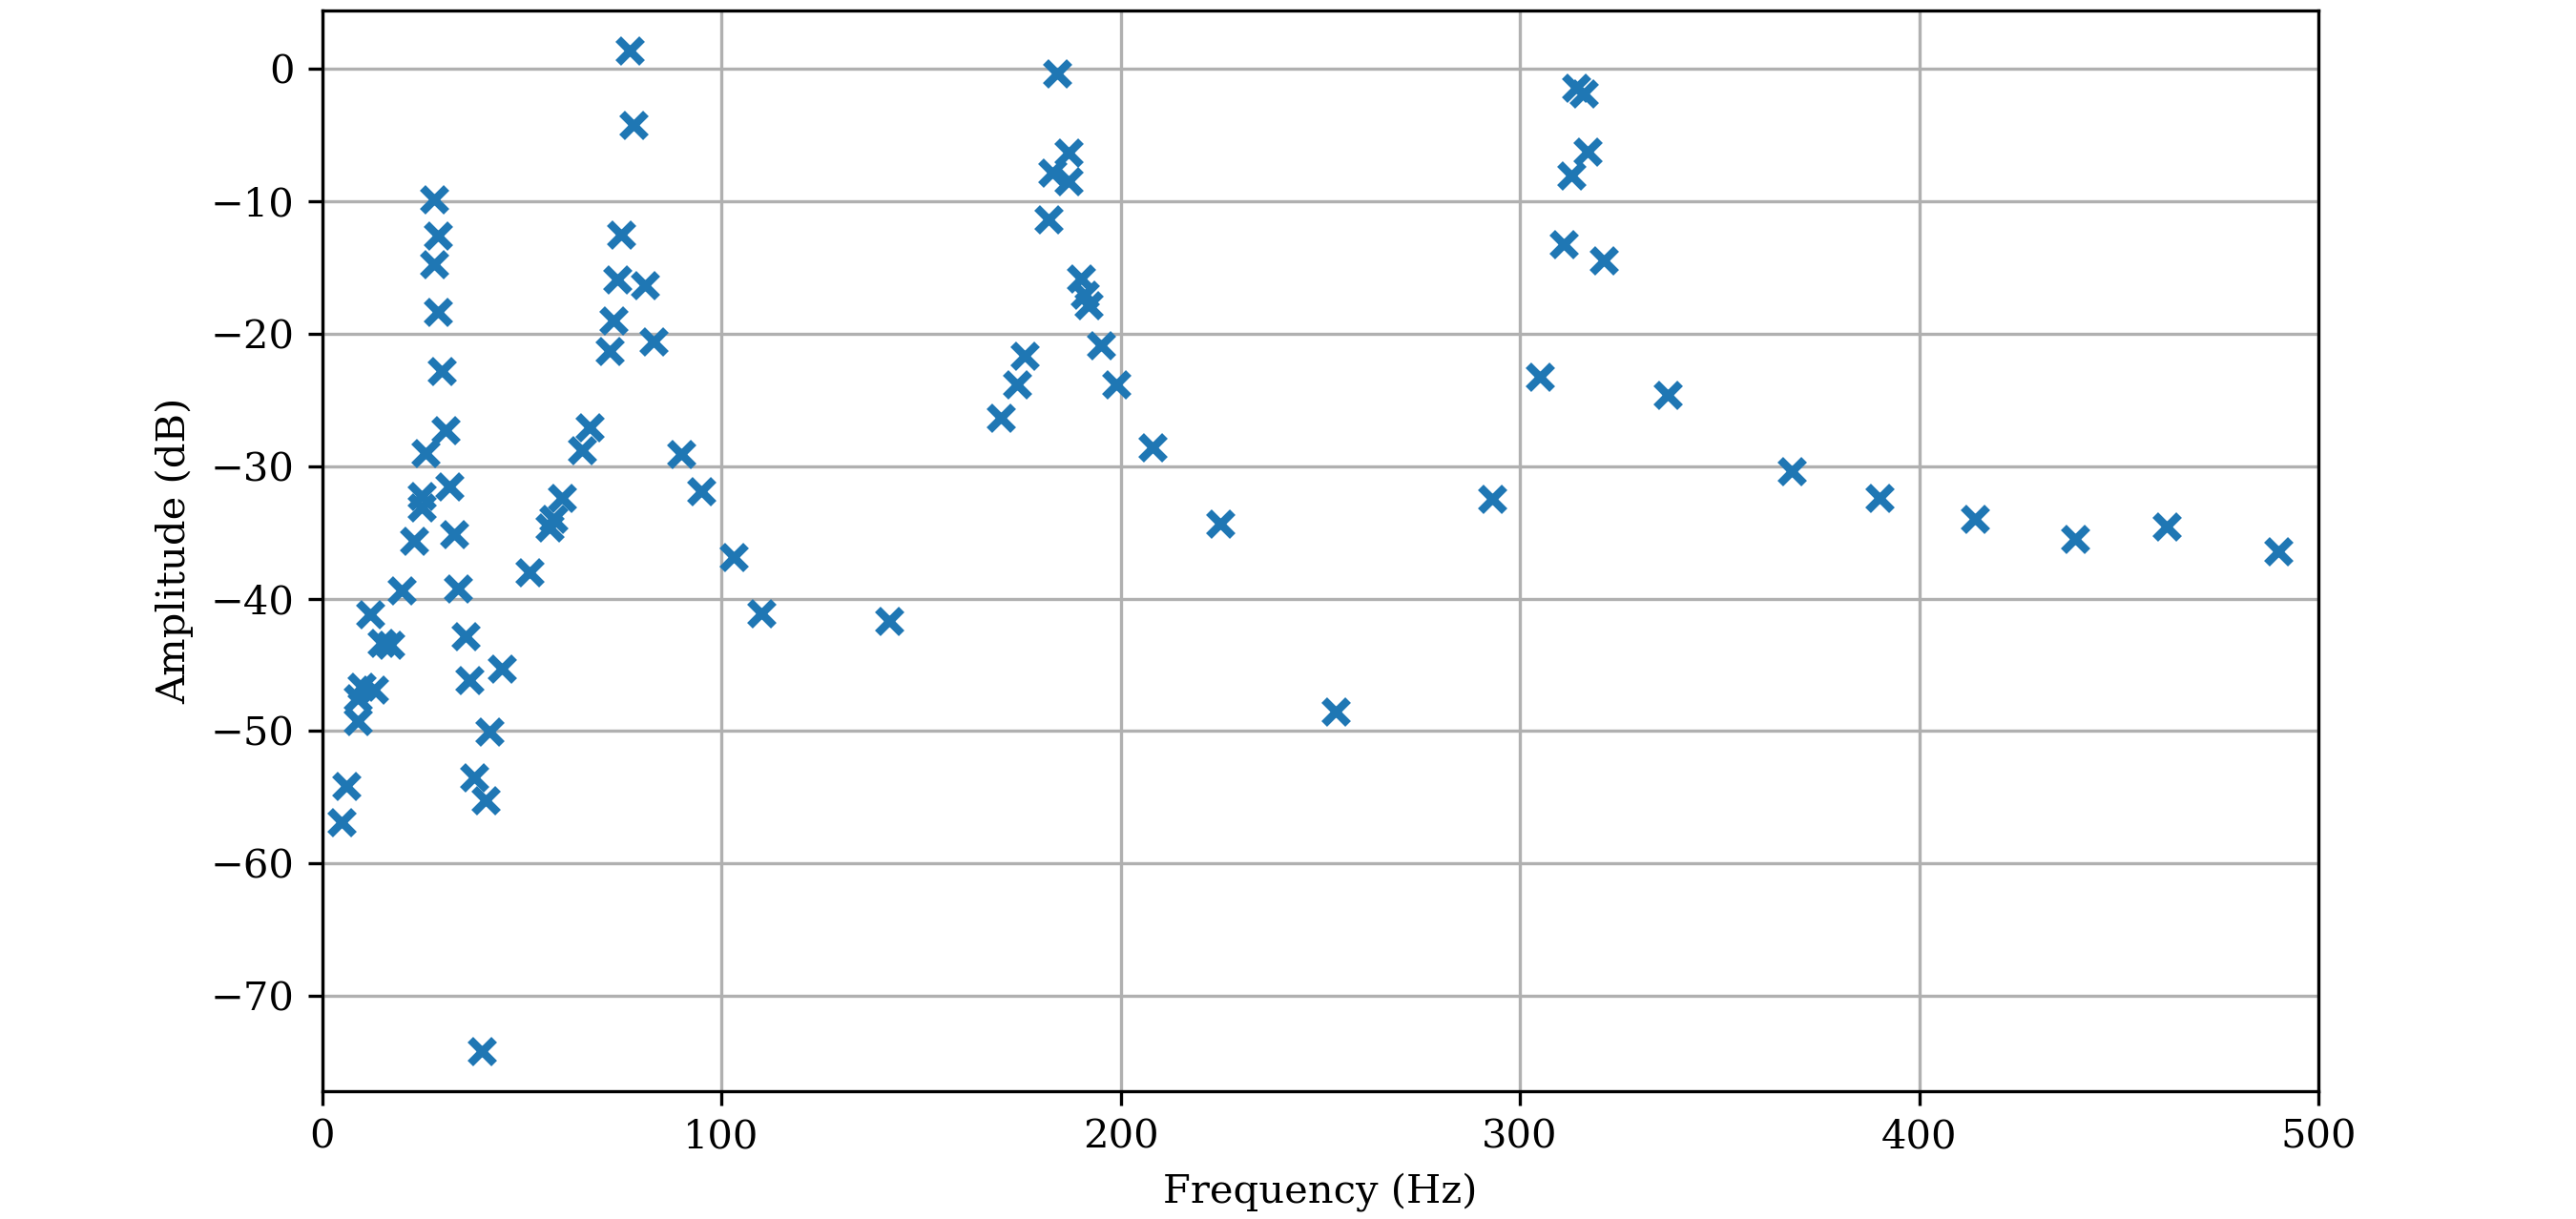
\includegraphics[width=\linewidth]{1-Sin}
  \caption{Transfer Function of a Sinusoidal input at frequencies up to 500Hz for the coupled beams}
  \label{fig:sin}
\end{figure}
%------------------------------------------------
\section{Results and Discussion}
\subsection{Sinusoidal Input}

Using a shaker and accelerometer the response to inputs at given frequencies can be measured and plotted see figure \ref{fig:sin}. Care must be taken to wait for the transient response to decay before each measurement. This is time consuming and difficult to accurately capture the whole behaviour close to resonances and anti-resonances. Four resonances were discovered at frequencies 25, 80, 190 and 310Hz. this process is usually automated with a generated frequency sweep. This would increase the speed considerably and give information on a range of desired frequencies reliably.


%--------------------------------------------------------------
\subsection{Random Noise Input}

\begin{figure}[!htb]
  \centering
    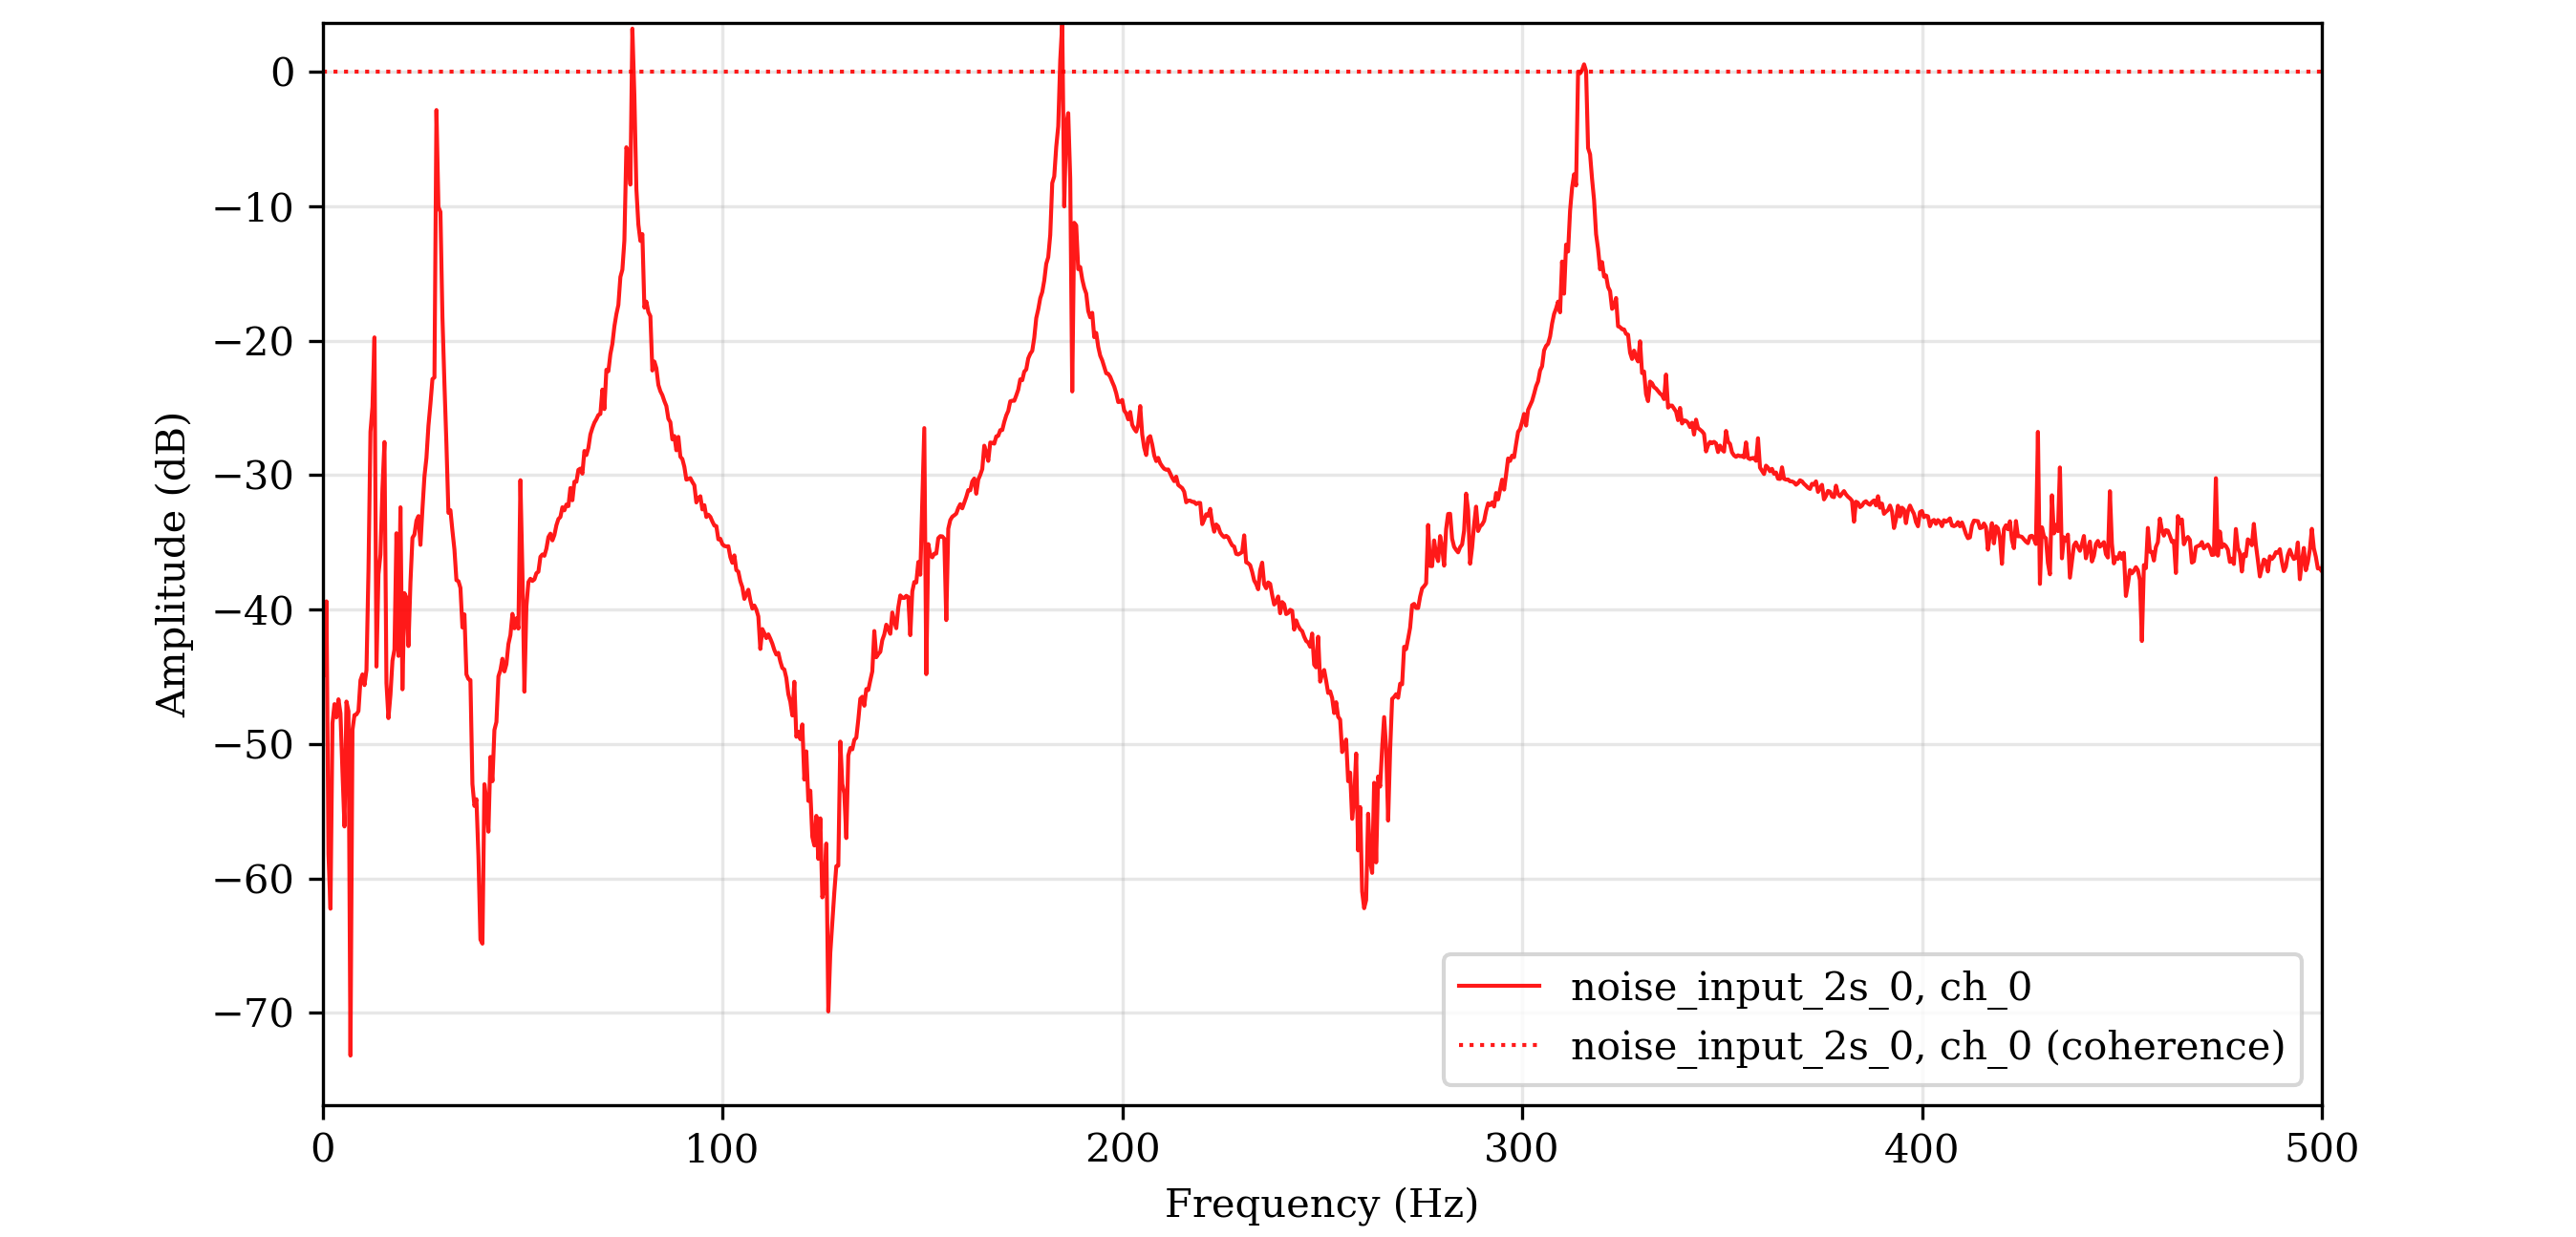
\includegraphics[width=\linewidth]{2-2snoiseTF}
  \caption{Transfer Function from a random noise signal generated for 2 seconds for coupled beams}
  \label{fig:n2tf}
\end{figure}
\begin{figure}[h]
  \centering
    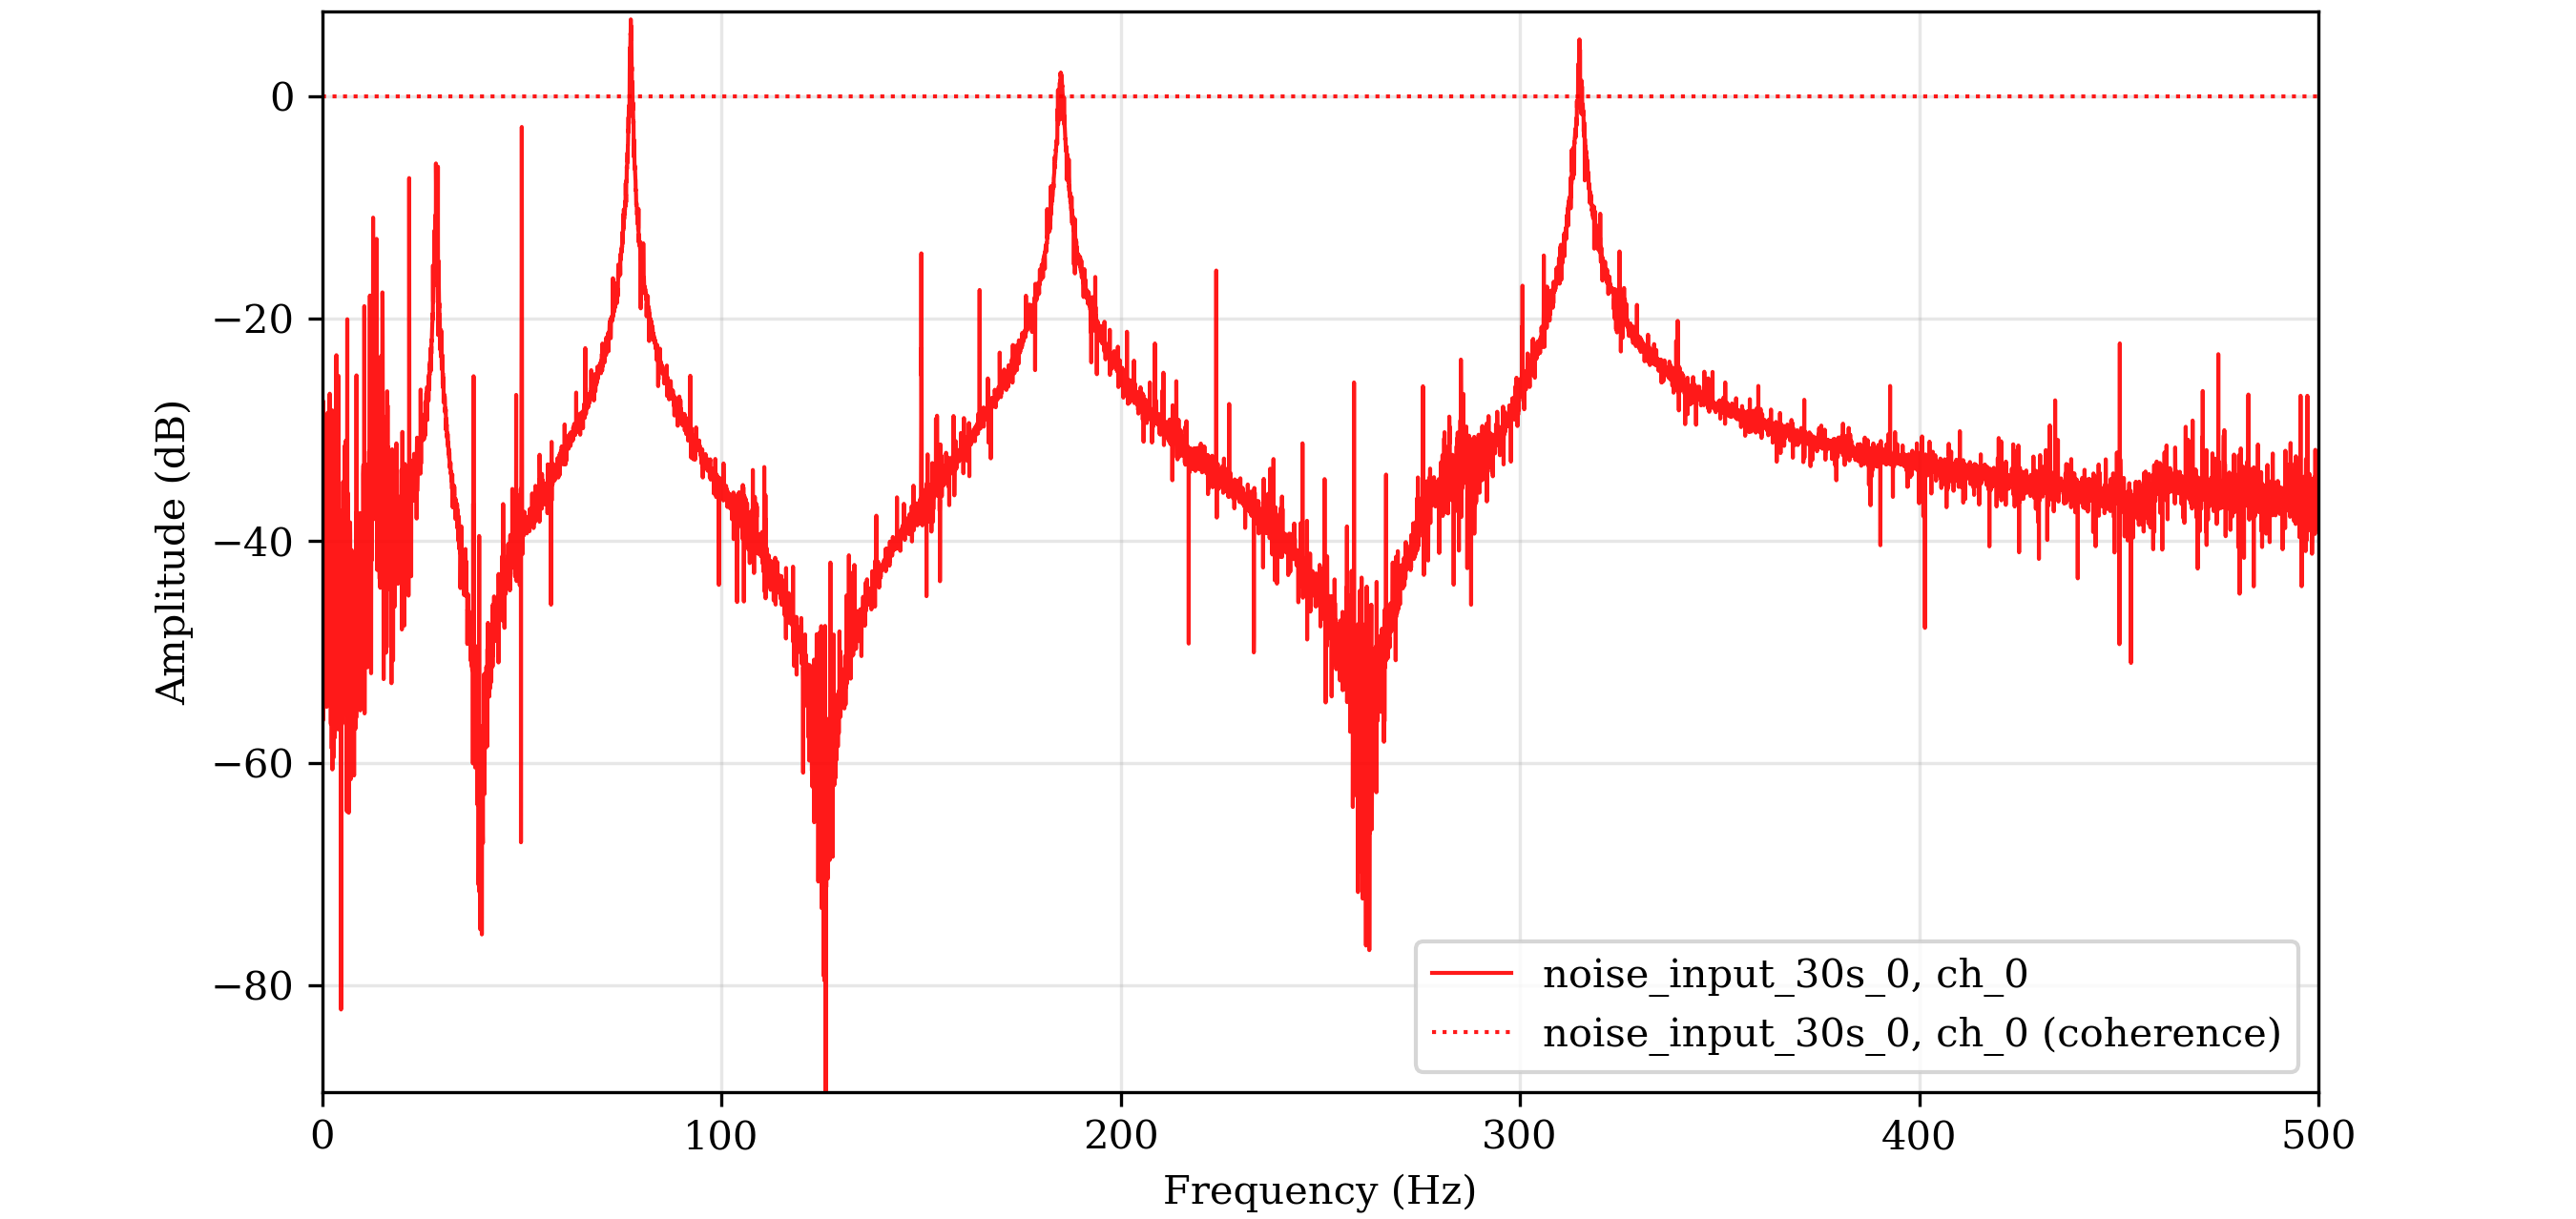
\includegraphics[width=\linewidth]{2-30snoiseTF}
  \caption{Transfer Function from a random noise signal generated for 30 seconds for coupled beams}
  \label{fig:n30tf}
\end{figure}

A faster method of obtaining the transfer function over a frequency range is to input a random noise force and sample over a time period, using Fourier analysis to separate the frequency responses. In order to represent the desired frequencies the sampling period must be long enough such that the frequencies of interest have been generated in the random noise input. Figures \ref{fig:n2tf} and \ref{fig:n30tf} show the transfer functions for 2s and 30s time periods. Both of these show the same four resonant peaks with the 30s time being slightly noisier. With the 30s time period peaks at 50Hz intervals can be seen which is the mains frequency. The low frequency 0-50Hz is far noisier due to accelerations being lower magnitude at low frequency, therefore sensitivity to measurement noise is high. A window can be used to reduce the noise of the transfer function. The window is applies in the time domain and ensures that both ends of the interval are zero magnitude. This means the signal is continuous in time when its periodically repeated, which is done during a FFT. The continuity creates a smoother transfer function as seen by comparing figures \ref{fig:n30tf} and \ref{fig:nowindow}.

\begin{figure}[!htb]
  \centering
    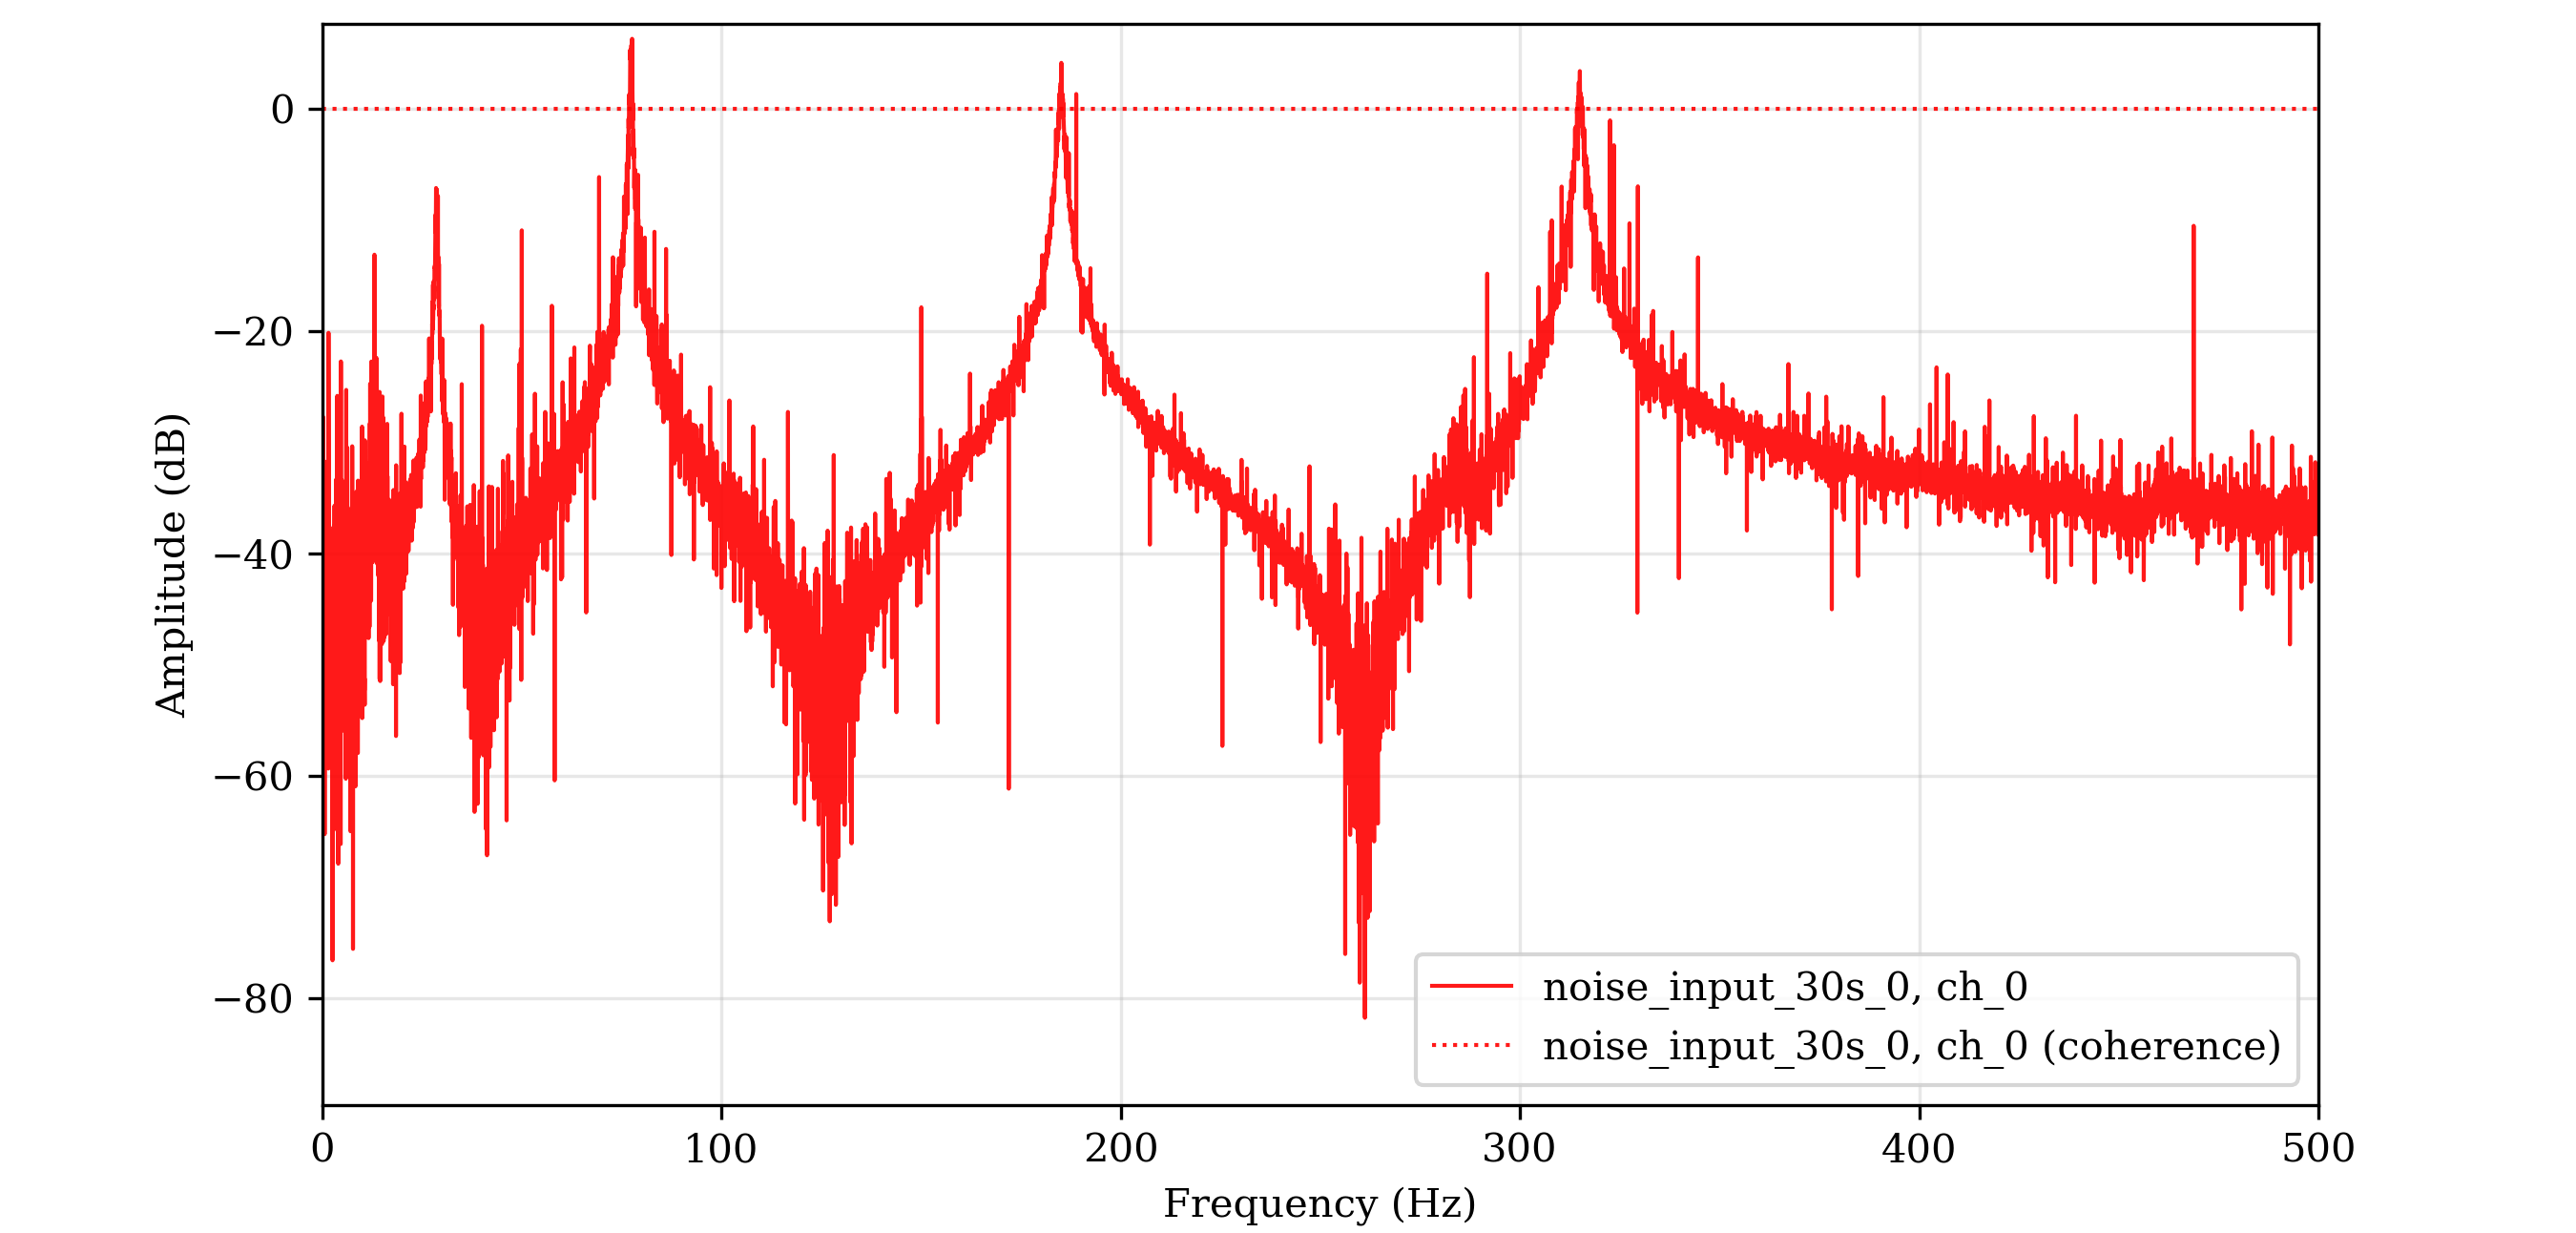
\includegraphics[width=\linewidth]{2-updatednowindow}
  \caption{Transfer Function without applying a window from a random noise signal generated for 30 seconds for coupled beams}
  \label{fig:nowindow}
\end{figure}


\begin{figure*}[t!]
    \centering
    \begin{subfigure}[t]{0.5\textwidth}
        \centering
        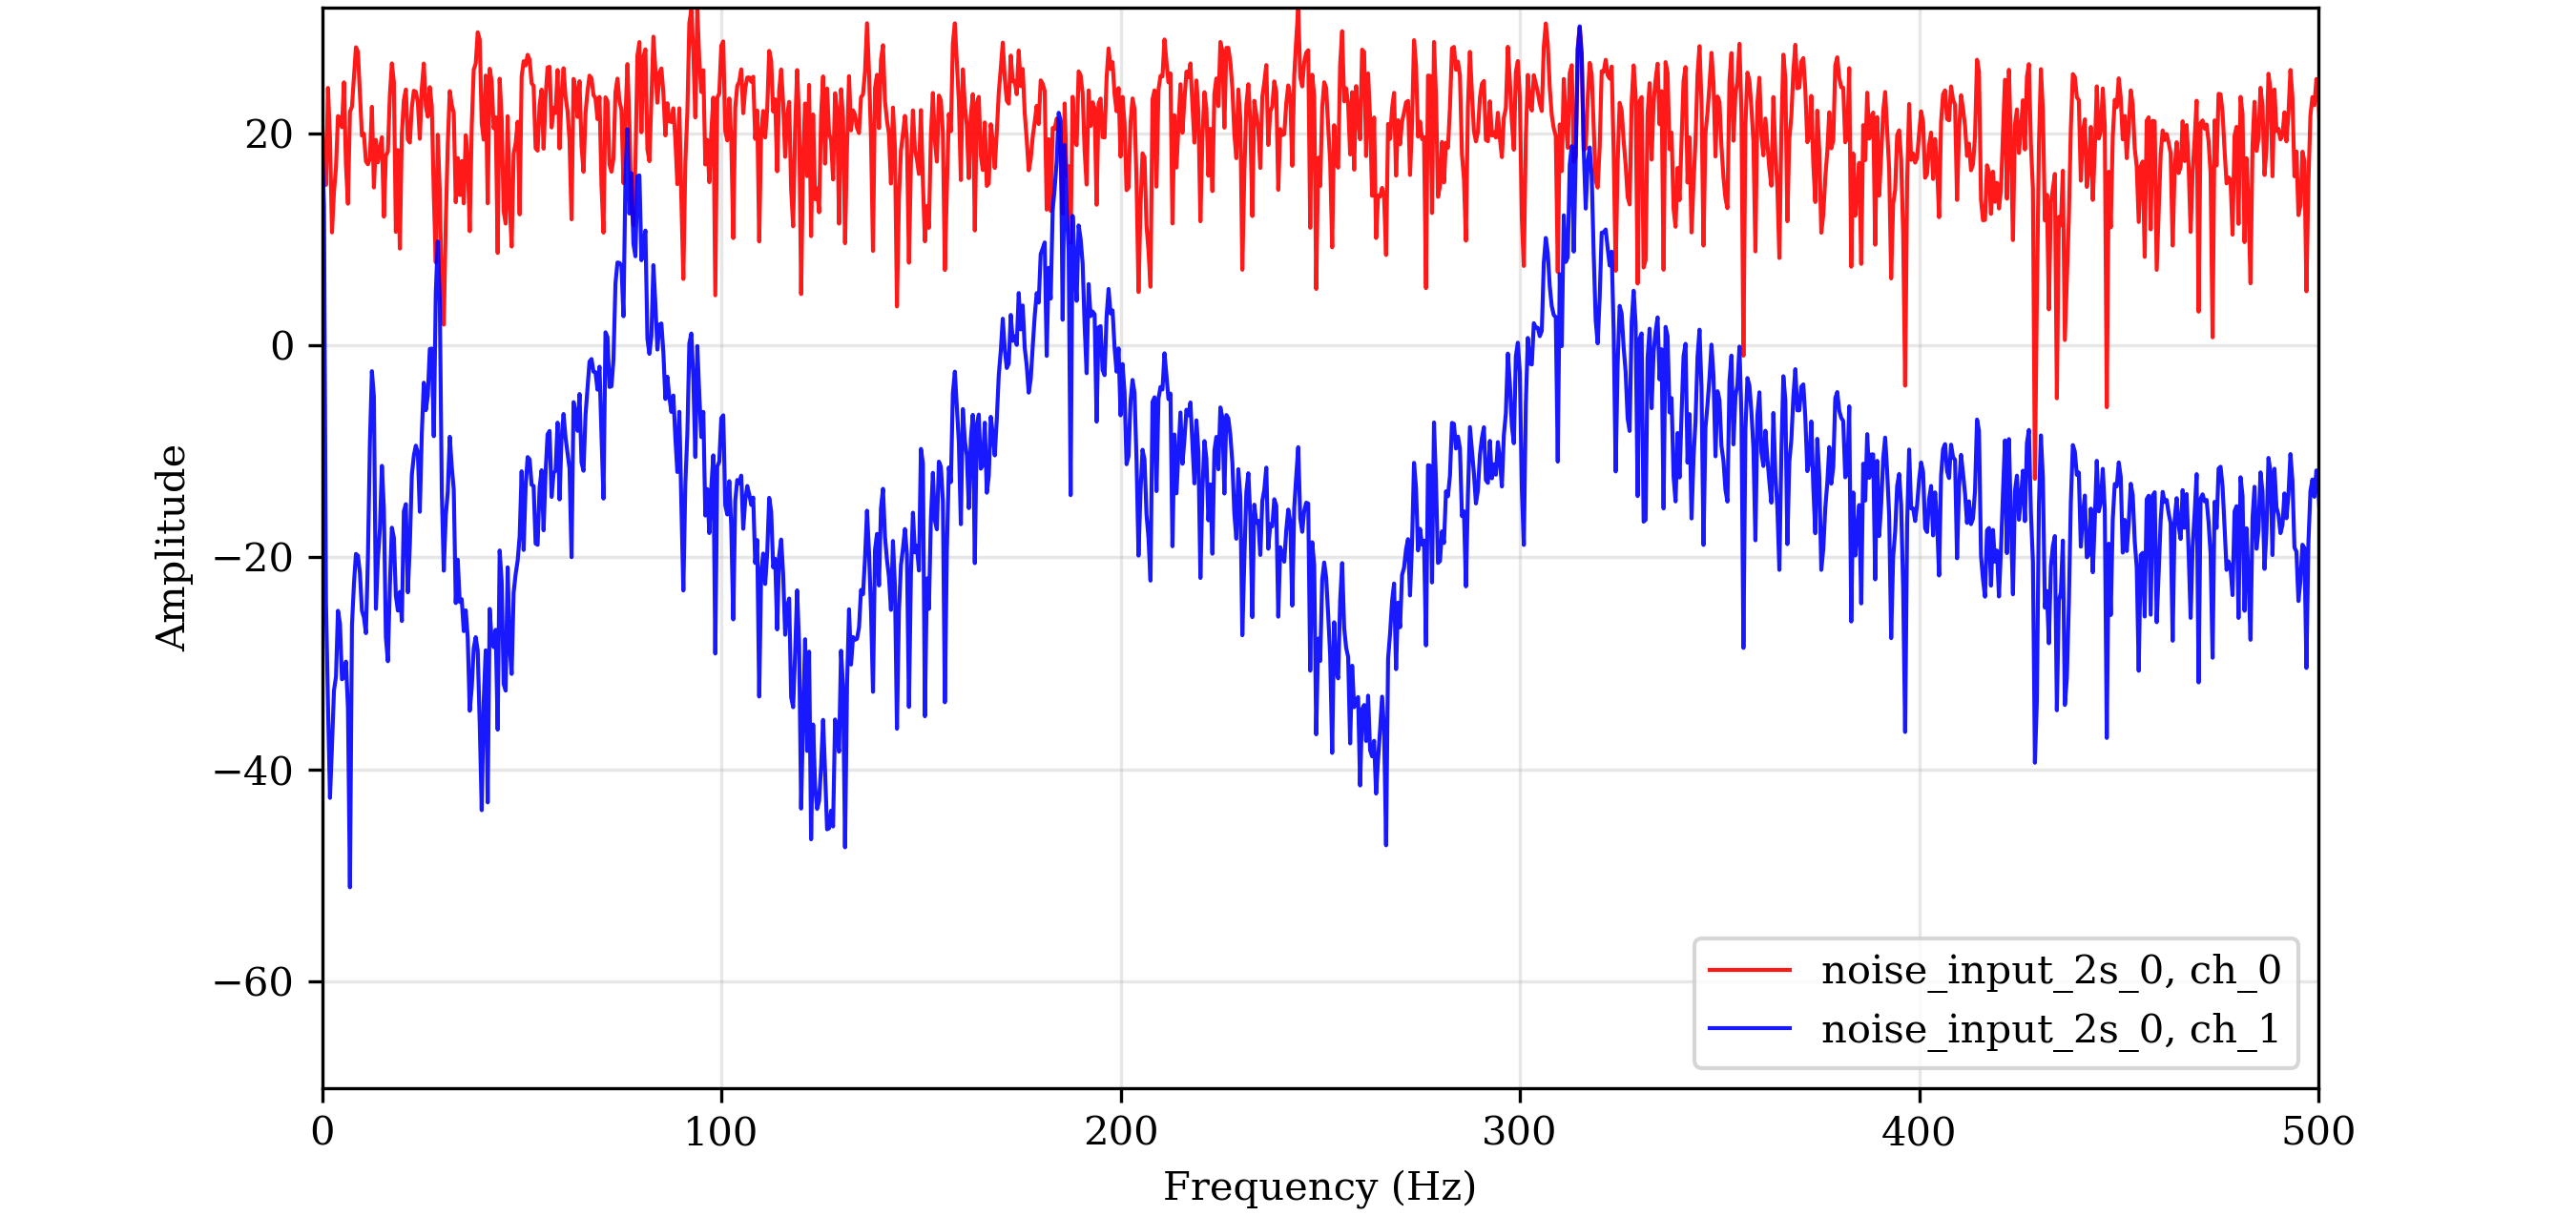
\includegraphics[height=1.55in]{2-2snoisefft}
        \caption{2 Seconds}
    \end{subfigure}%
    ~ 
    \begin{subfigure}[t]{0.5\textwidth}
        \centering
        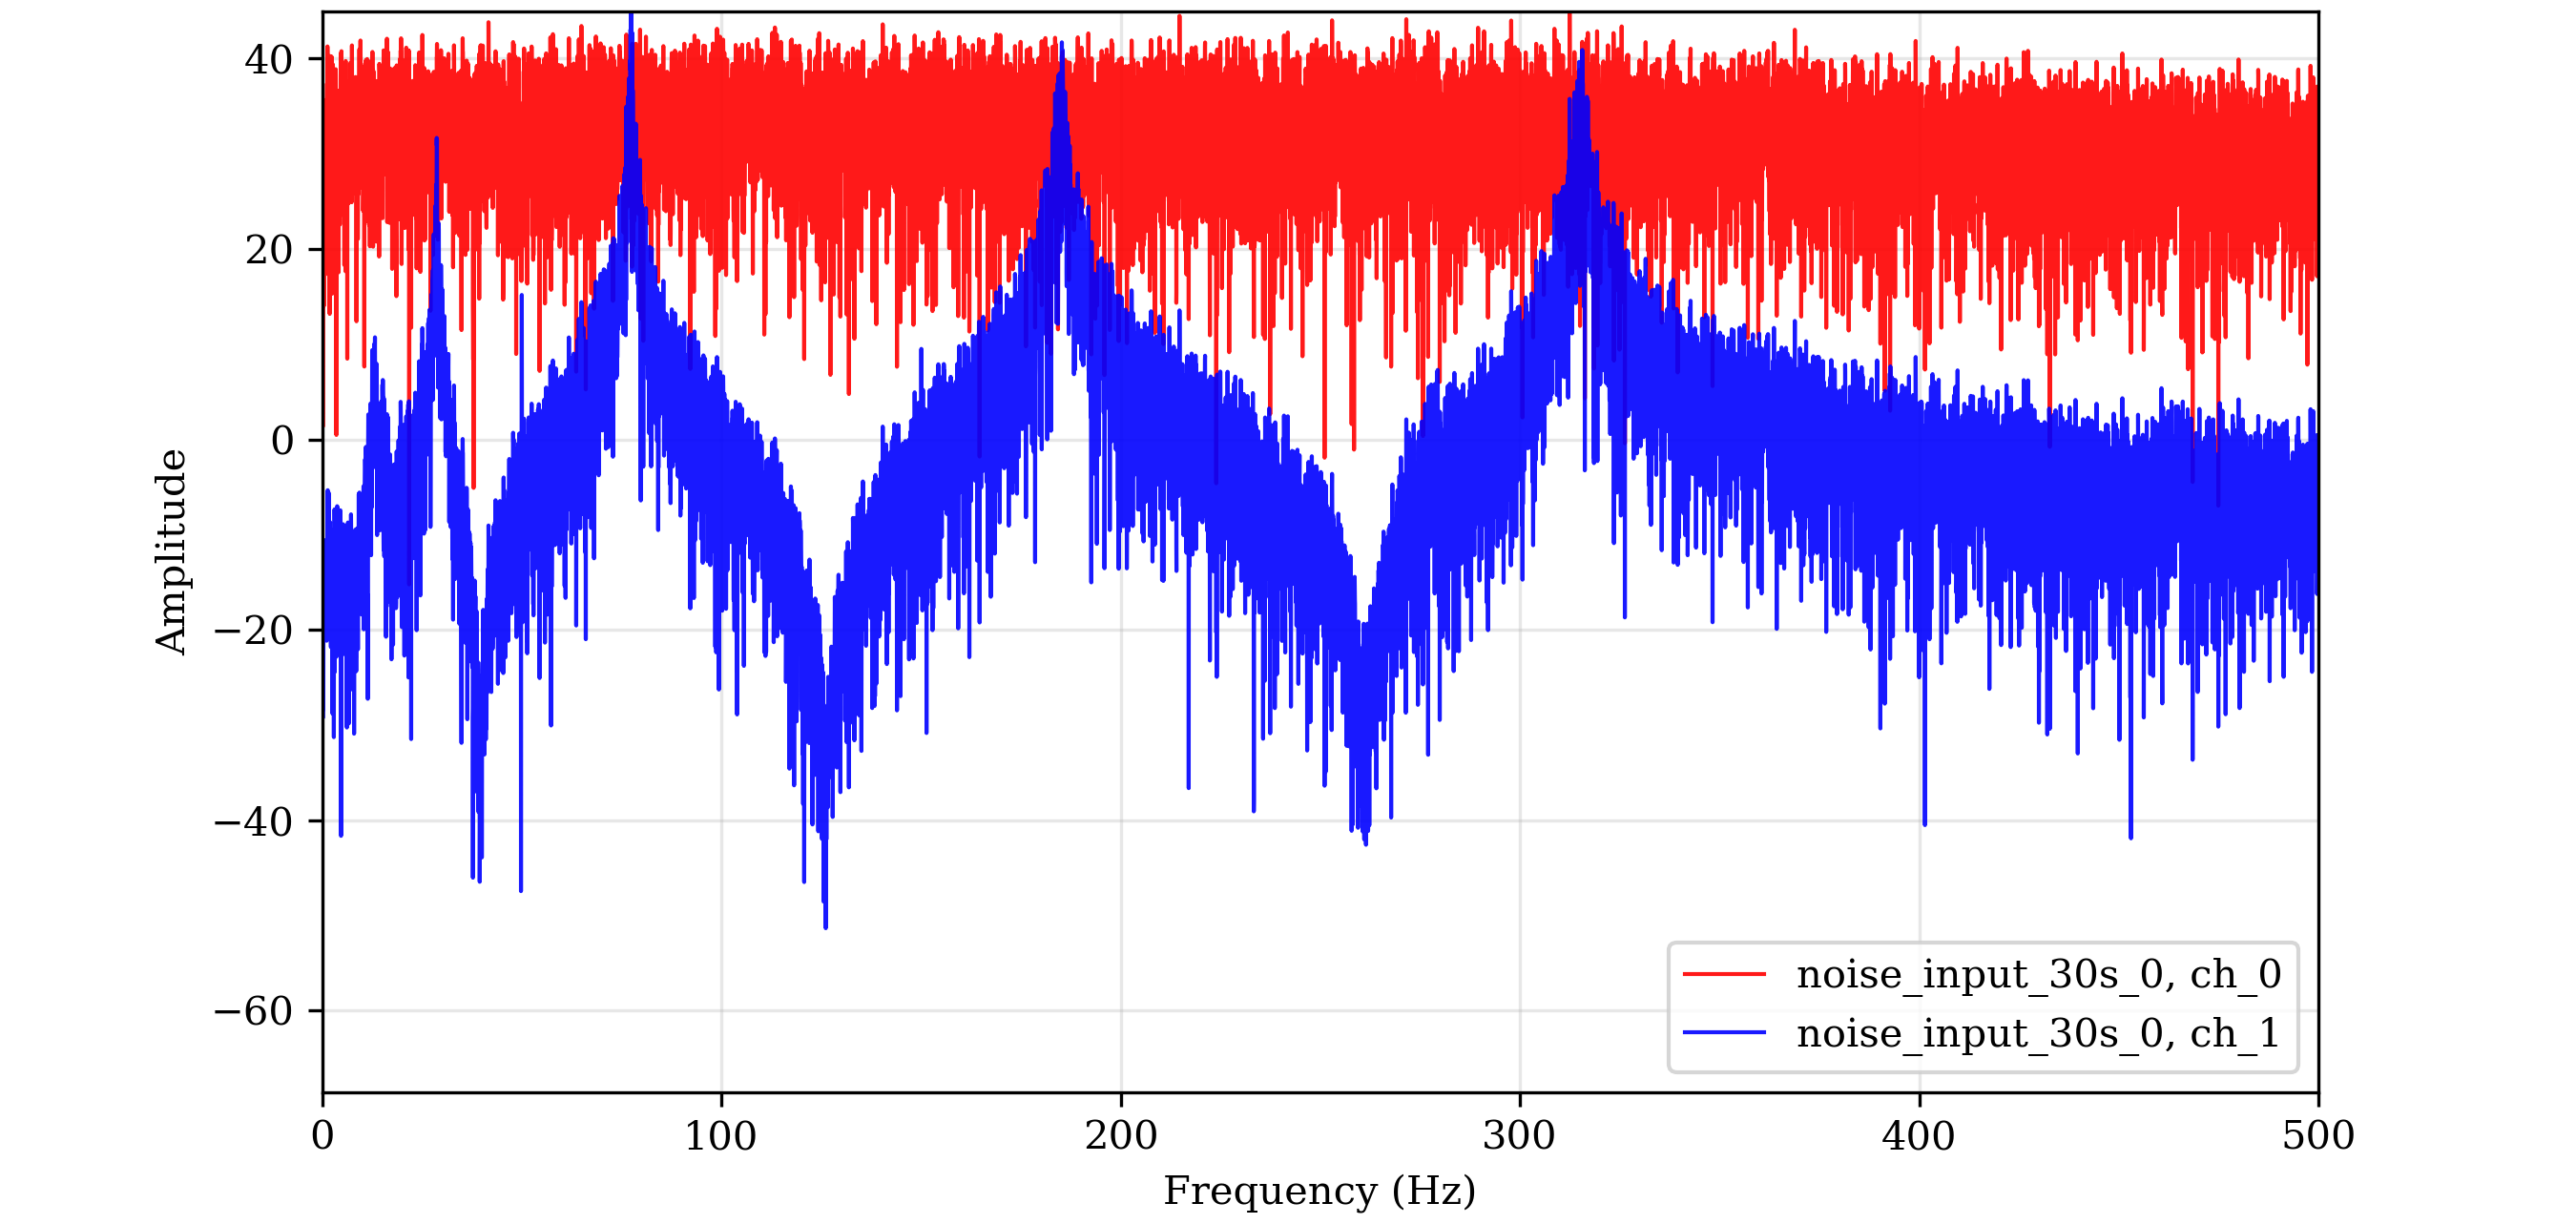
\includegraphics[height=1.55in]{2-30snoisefft}
        \caption{30 Seconds}
    \end{subfigure}
    \caption{Fast Fourier Transform from a random noise signal generated for 2 and 30 seconds on coupled beams}
    \label{fig:2ffts}
\end{figure*}


Figure \ref{fig:2ffts} shows the FFTs of the noise inputs (red) and response (blue). The larger sampling period shows better frequency resolution across the range. However, the variance in magnitude across these frequencies is larger than the smaller interval thus creating the noisier transfer function.

\begin{figure}[!hb]
  \centering
    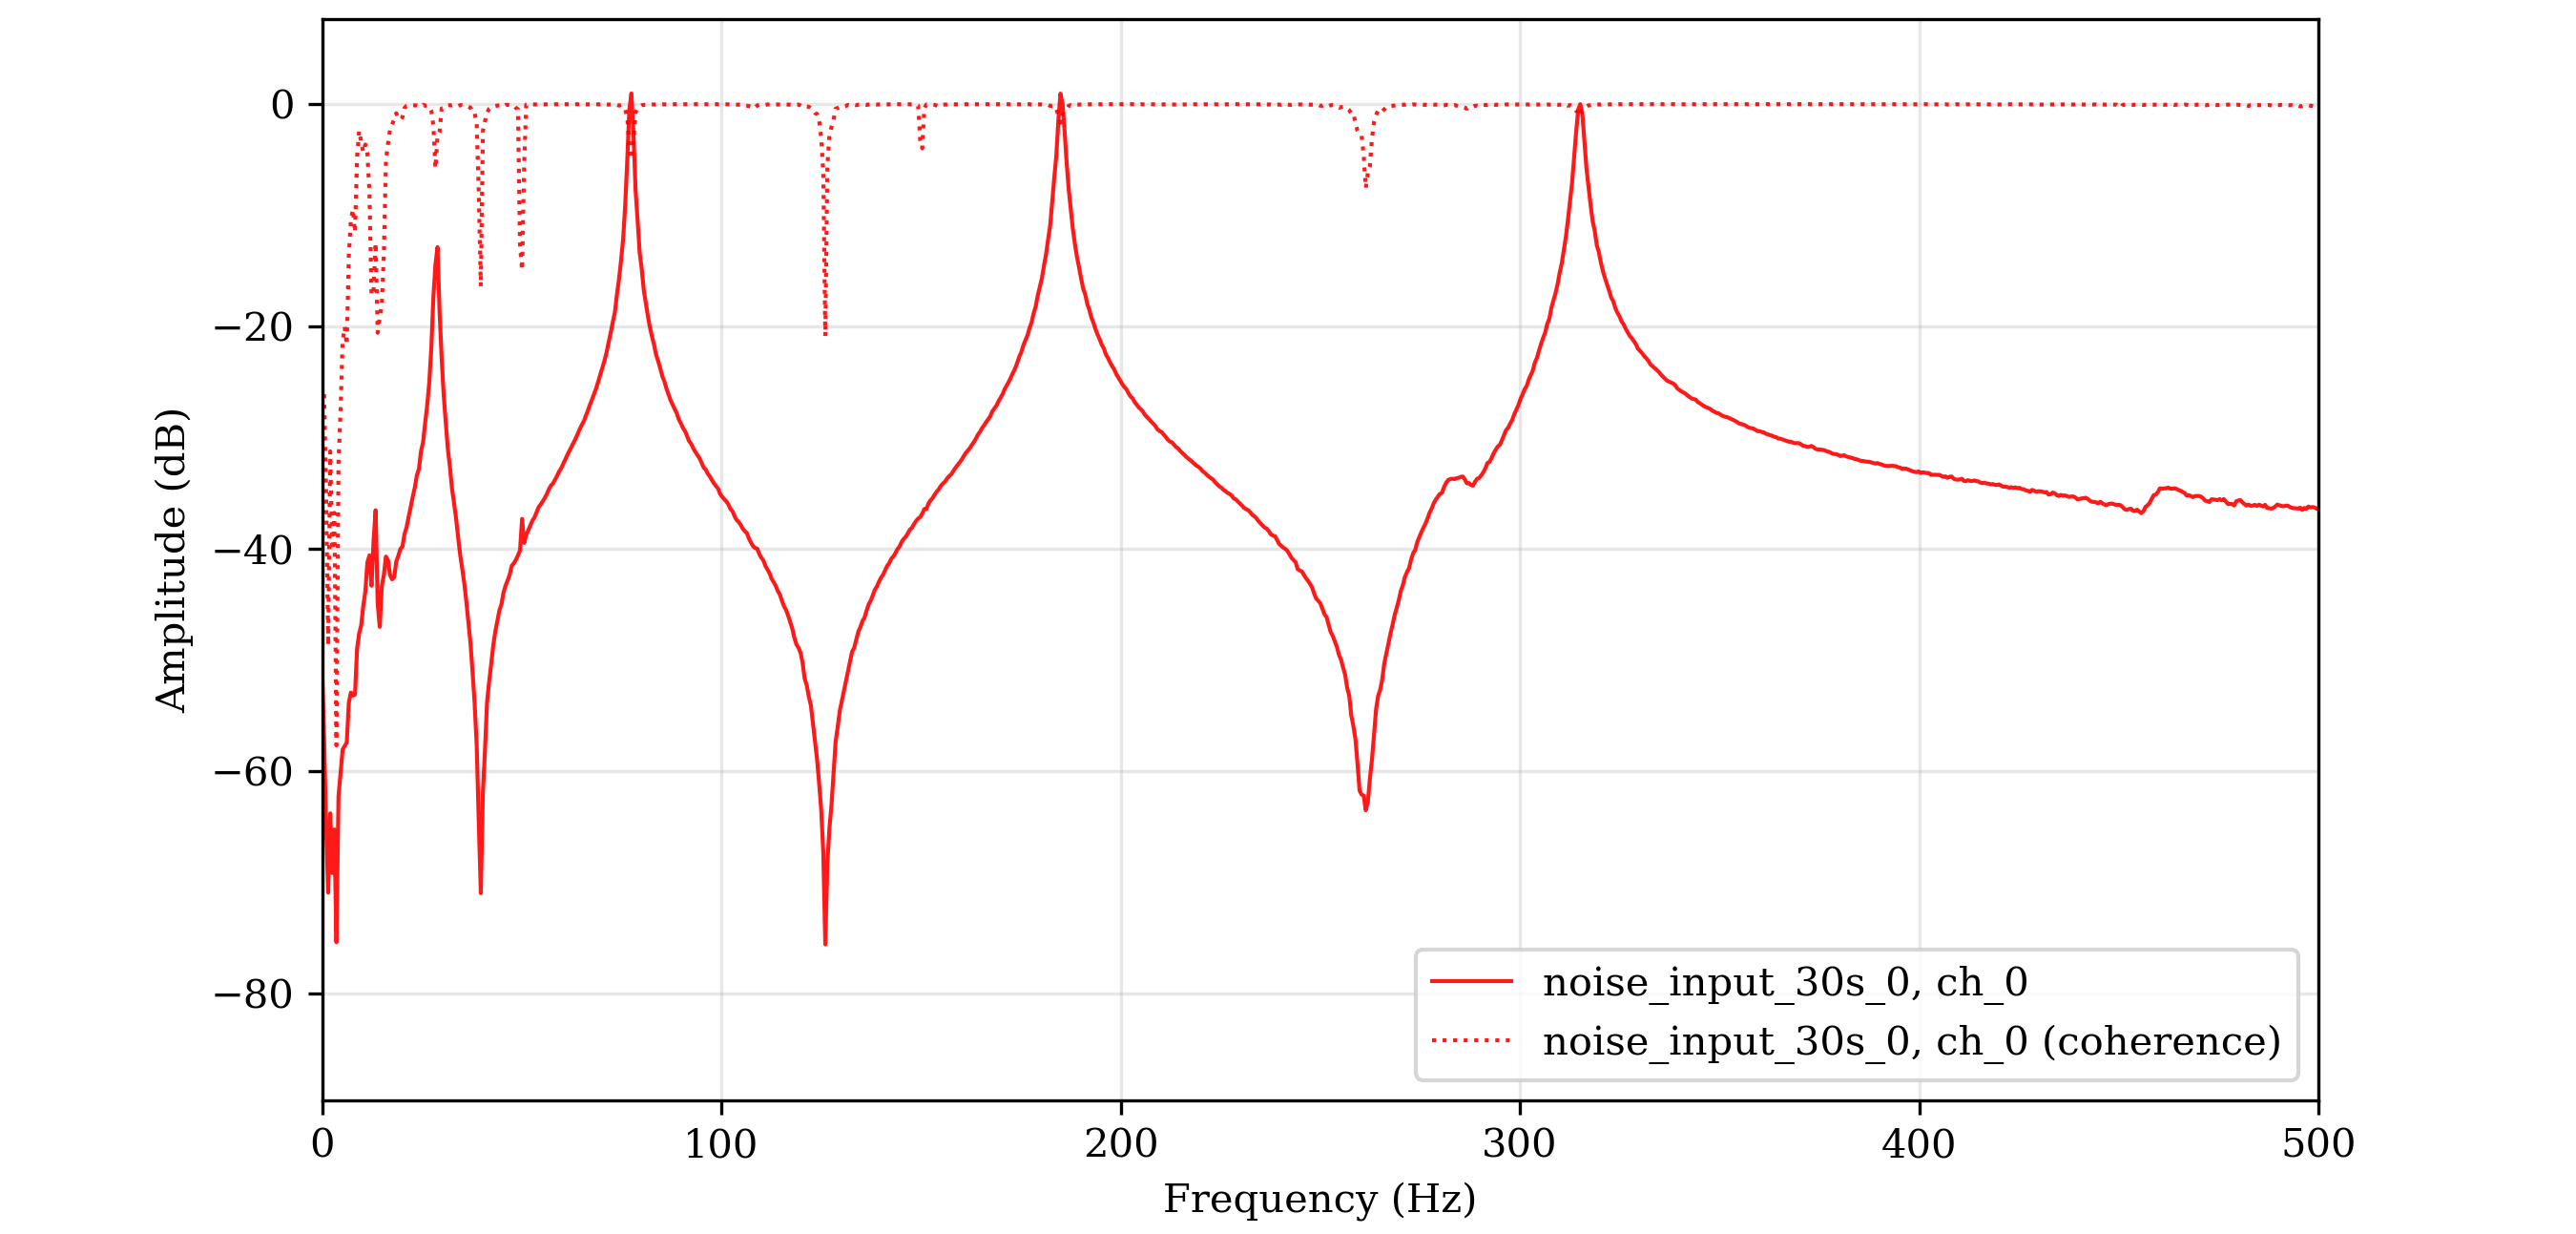
\includegraphics[width=\linewidth]{2-n=30}
  \caption{Transfer function with a noise input with 30, 1s time intervals averaged}
  \label{fig:n=30}
\end{figure}

\begin{figure}[h]
  \centering
    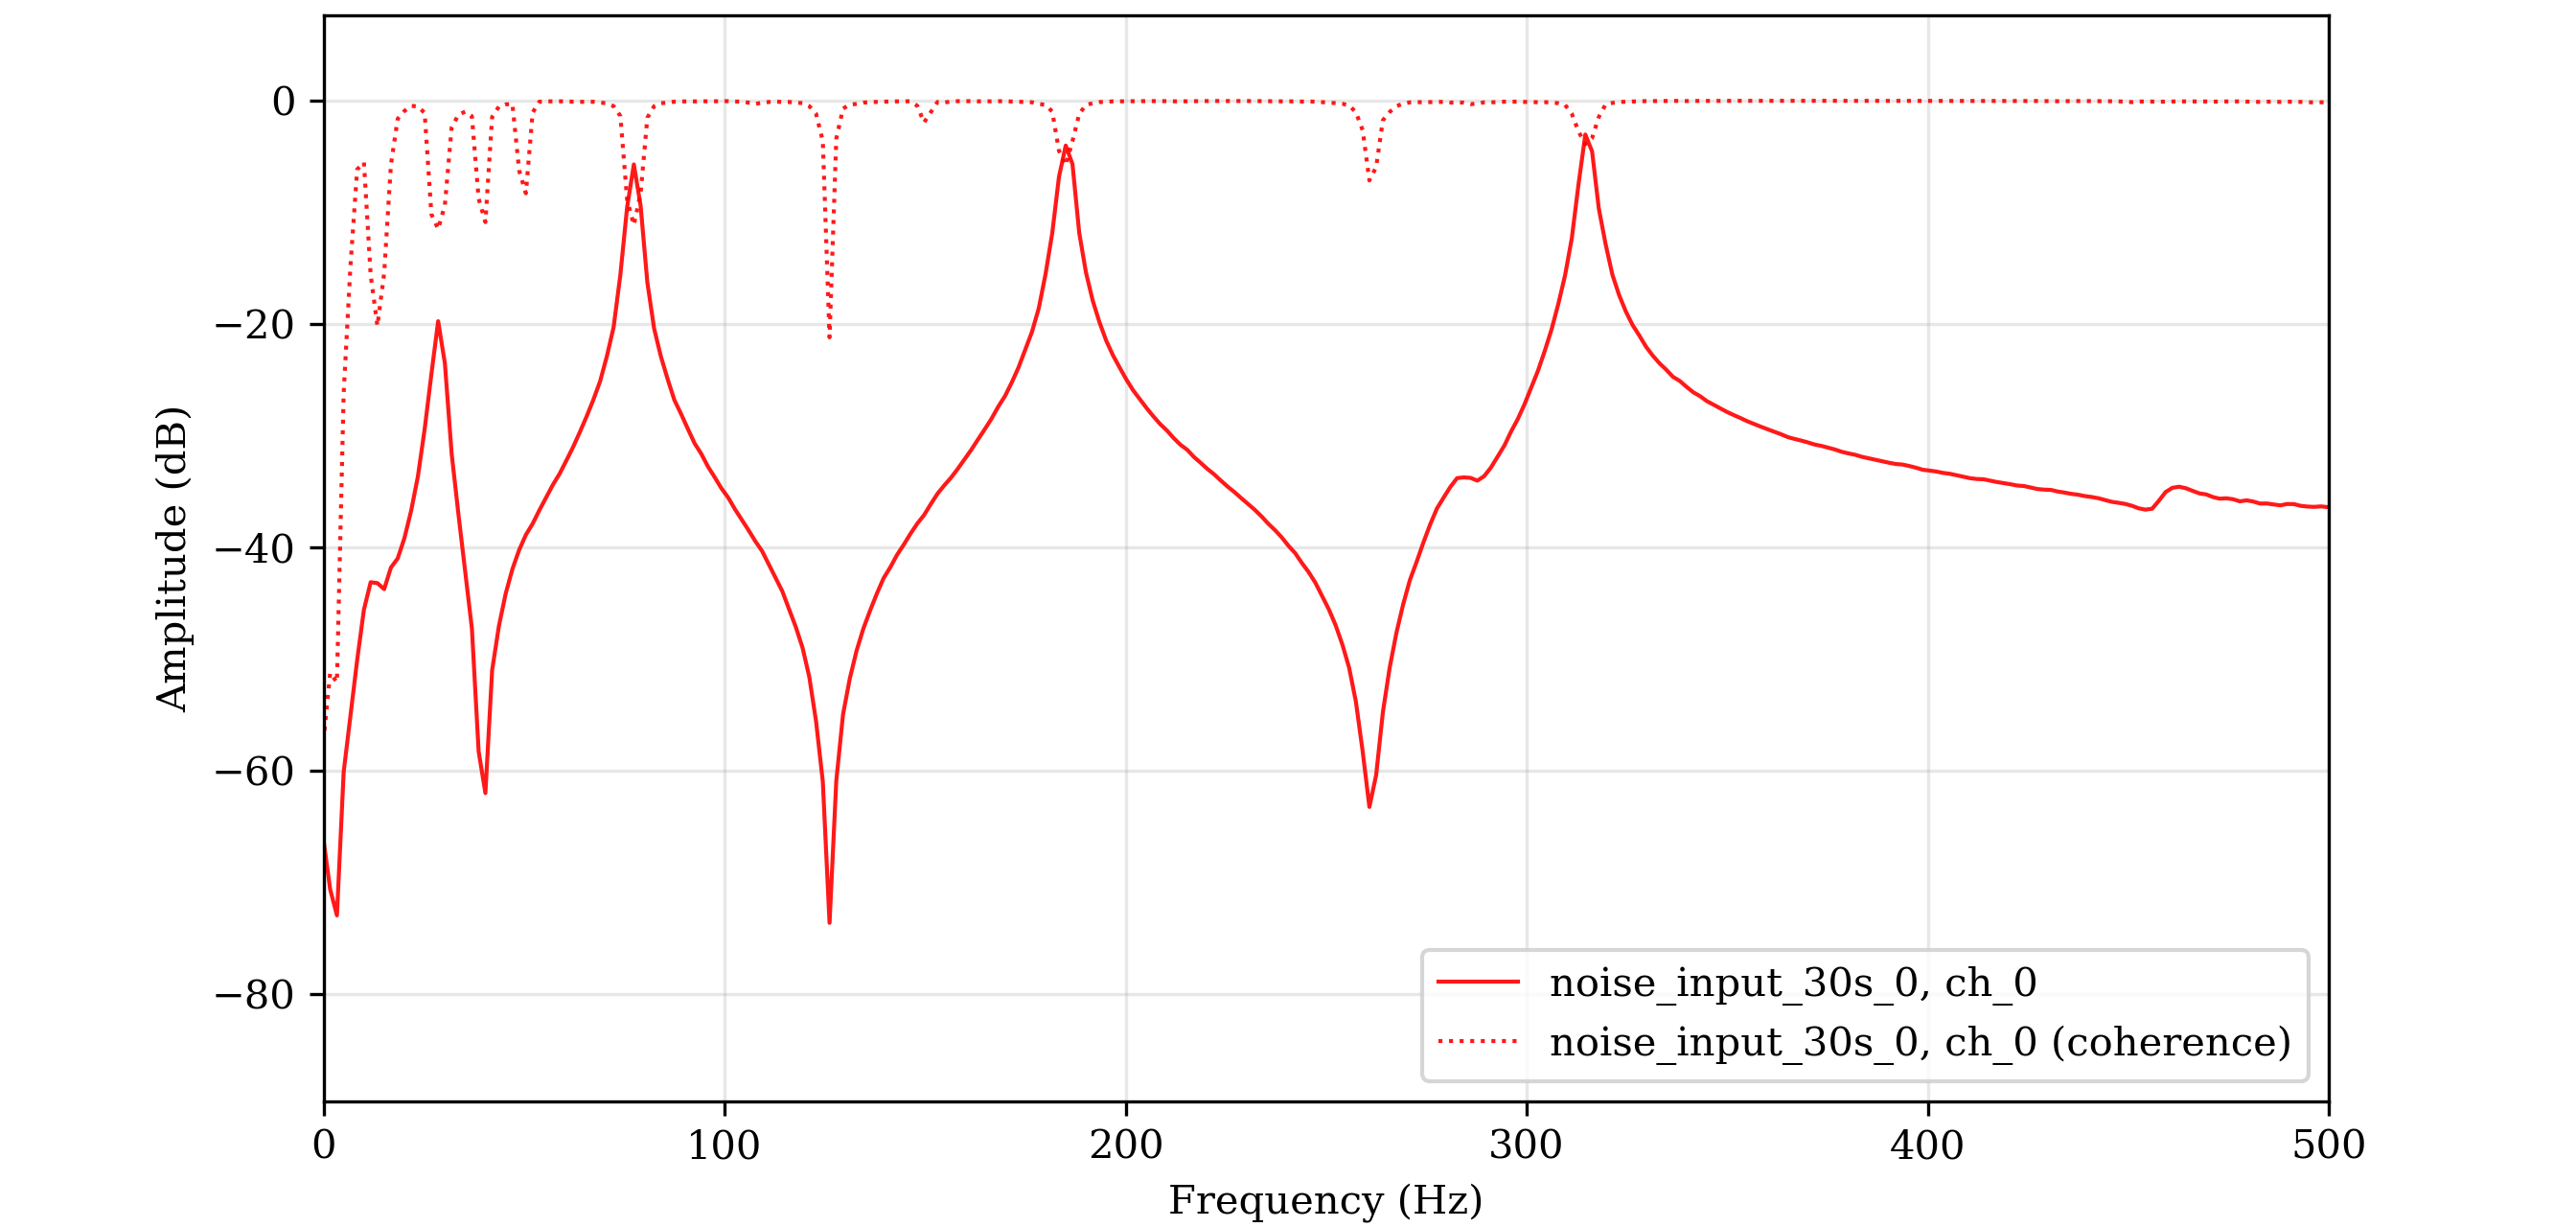
\includegraphics[width=\linewidth]{2-n=100}
  \caption{Transfer function with a noise input with 100, 0.3s time intervals averaged}
  \label{fig:n=100}
\end{figure}

The noise present in the transfer function can be reduced by splitting up the whole interval of 30s into n intervals, performing a FFT on each mini interval and then averaging. The result of this for n=1, 30 and 100 can be seen in figures \ref{fig:n30tf} , \ref{fig:n=30} and \ref{fig:n=100} respectively. Care must be taken as using too many intervals means that the each interval will have lower frequency resolution. Additionally a lack of causality can be introduced as the input during one interval will cause an output in following intervals. This means input and output response can't be matched correctly within one interval and accuracy is lost. The reduced coherence between averaged results which can be seen at resonances in figure \ref{fig:n=100} for n=100. When n=30 the transfer function has good coherence at points of interest such as resonance, and the noise has been eliminated as desired. Incoherent results are to be expected at anti-resonances and very low frequencies as these have lower accelerations so are more sensitive to measurement noise.
%--------------------------------------------------------------
\subsection{Hammer Input}
\begin{figure}[!hb]
  \centering
    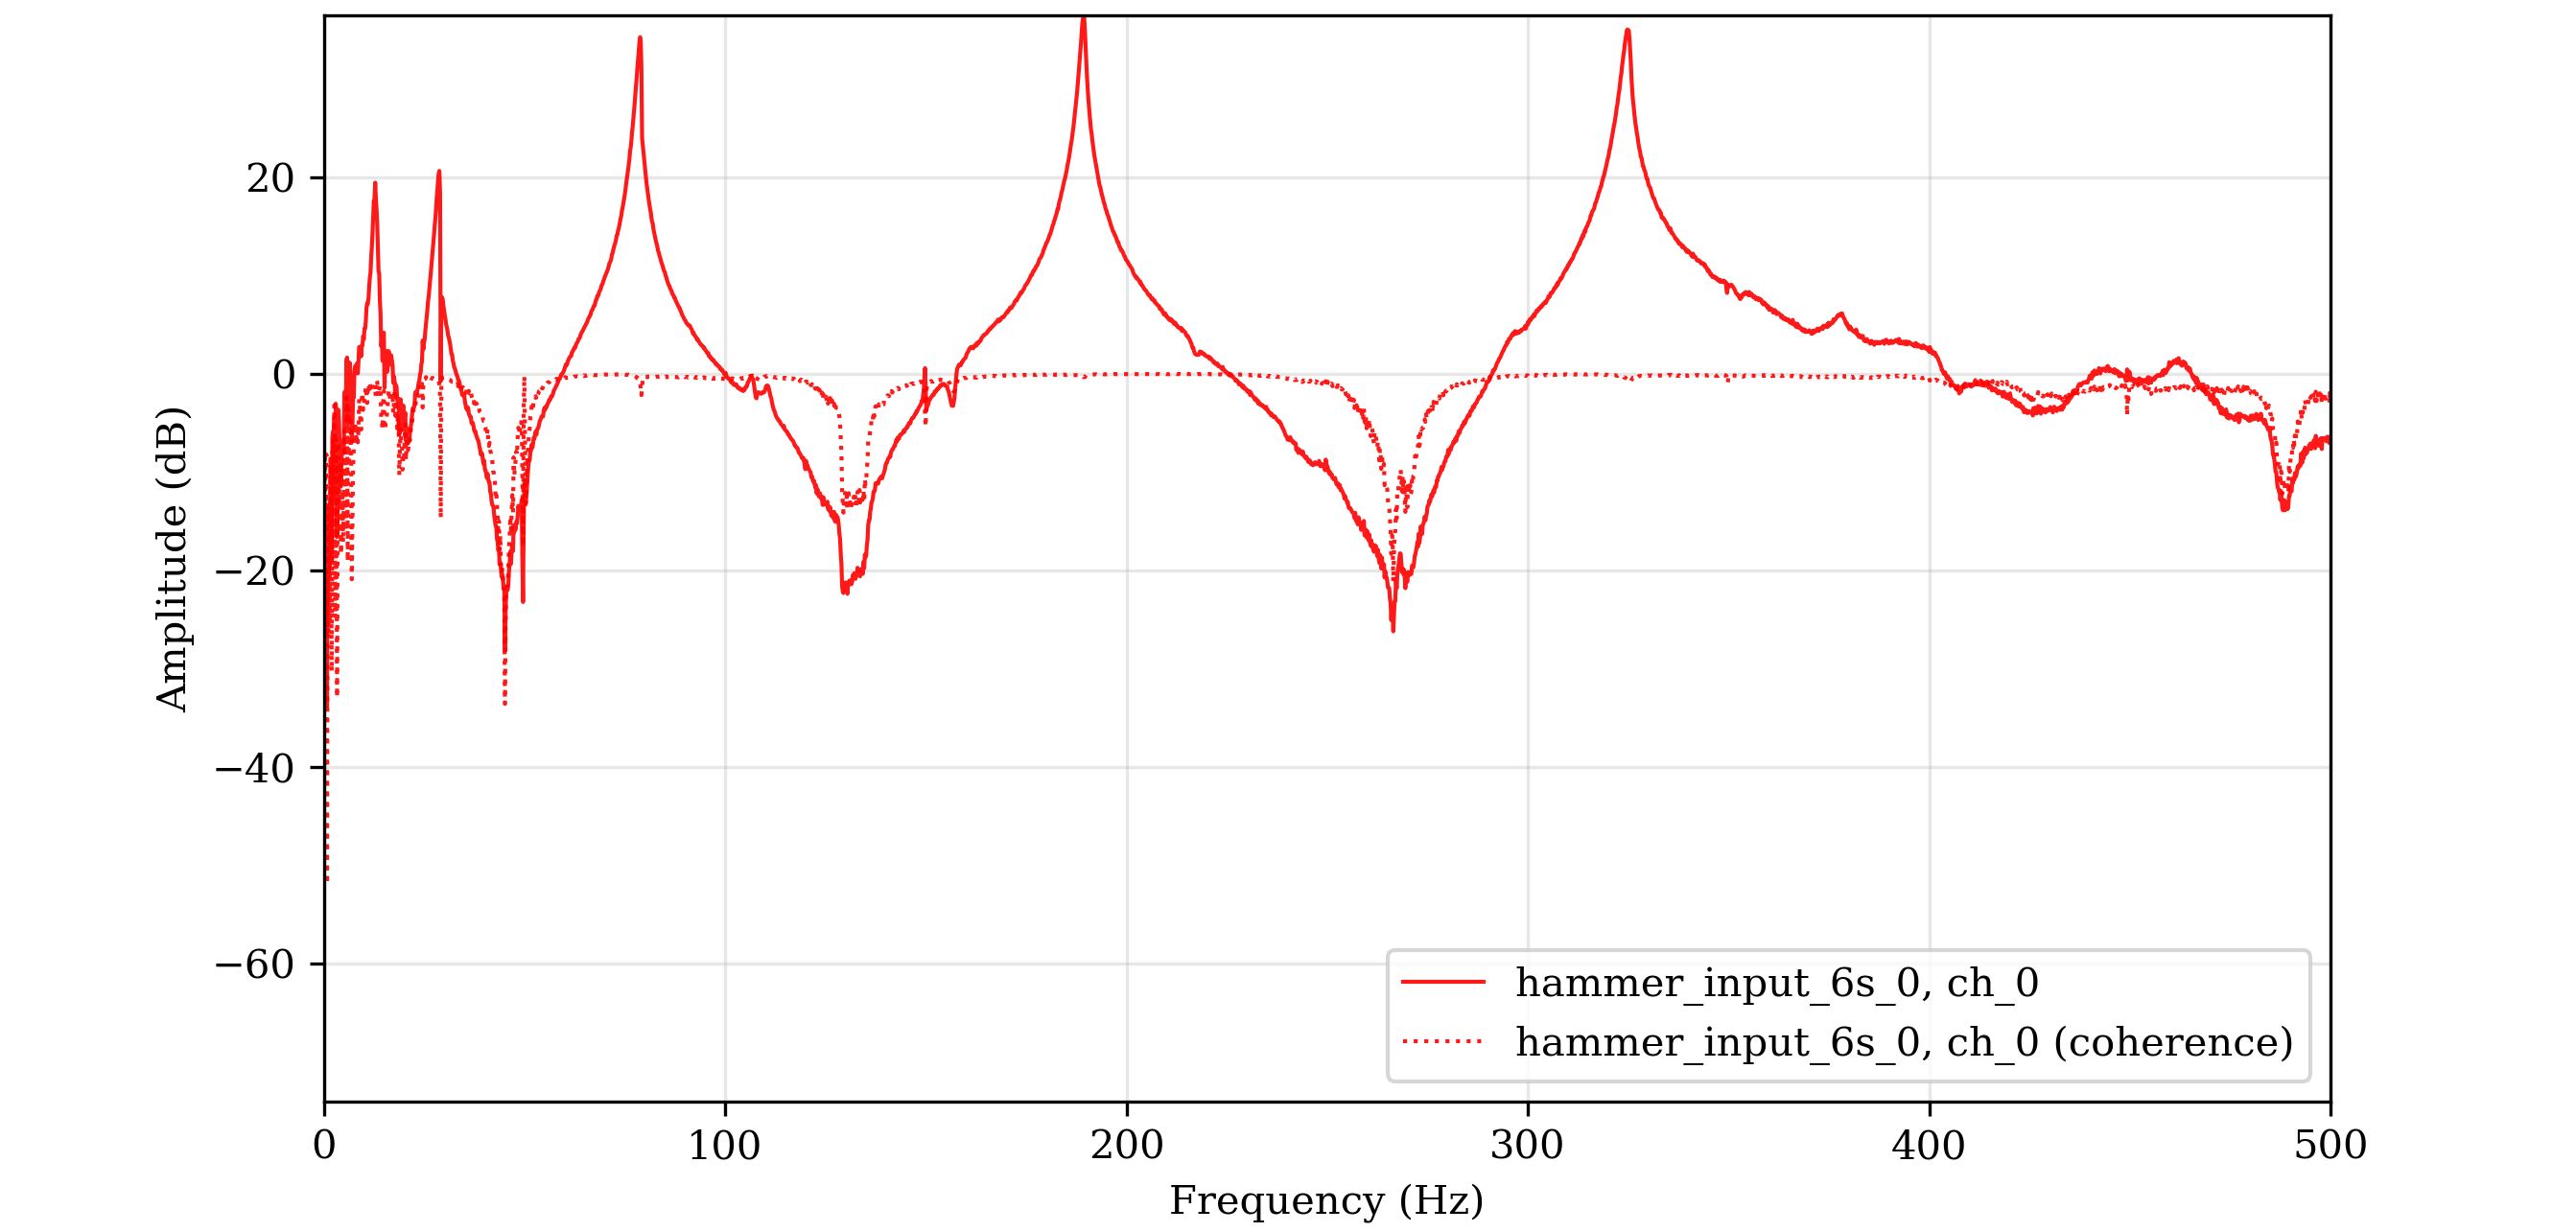
\includegraphics[width=\linewidth]{3-hammertf}
  \caption{Transfer Function due to an impulse from a hammer  for coupled beams}
  \label{fig:htf}
\end{figure}



A third method to obtain the transfer function is to excite the structure with an impulse and measure the response. The frequencies being tested can be found by doing a Fourier transform on the shape of the force input. For an ideal impulse this will include all frequencies. However, a hammer strike produces a more rounded force input due to a finite contact time therefore the higher frequencies aren't present, figure \ref{fig:impulse} shows the decay of the frequencies present in the input. A longer hammer pulse causes the frequency cutoff to occur at a lower value. A window isn't required in the method to obtain a smooth transfer function, the window would actually reduce all useful data to zero. Figure \ref{fig:htf} shows the transfer function of five hits averaged together. Five peaks can be seen in this plot. This additional peak is due a rigid body motion of the structure vibrating on the rubber supports, therefore isn't a true mode as its cause is the experimental set-up. This occurs at a low frequency of 20Hz as a large mass is moving with low stiffness opposing motion, therefore a low frequency is expected. This mode didn't occur using  other measurements techniques as the cause of this mode is an external force input. The shaker exited the structure from internally so is unable to cause this motion on the rubber feet. Coherence between tests needs to be high at frequencies of interest about the resonances. The coherence is lower at very low frequencies and around antiresonance's due to lower accelerations.


\begin{figure}[!htb]
  \centering
    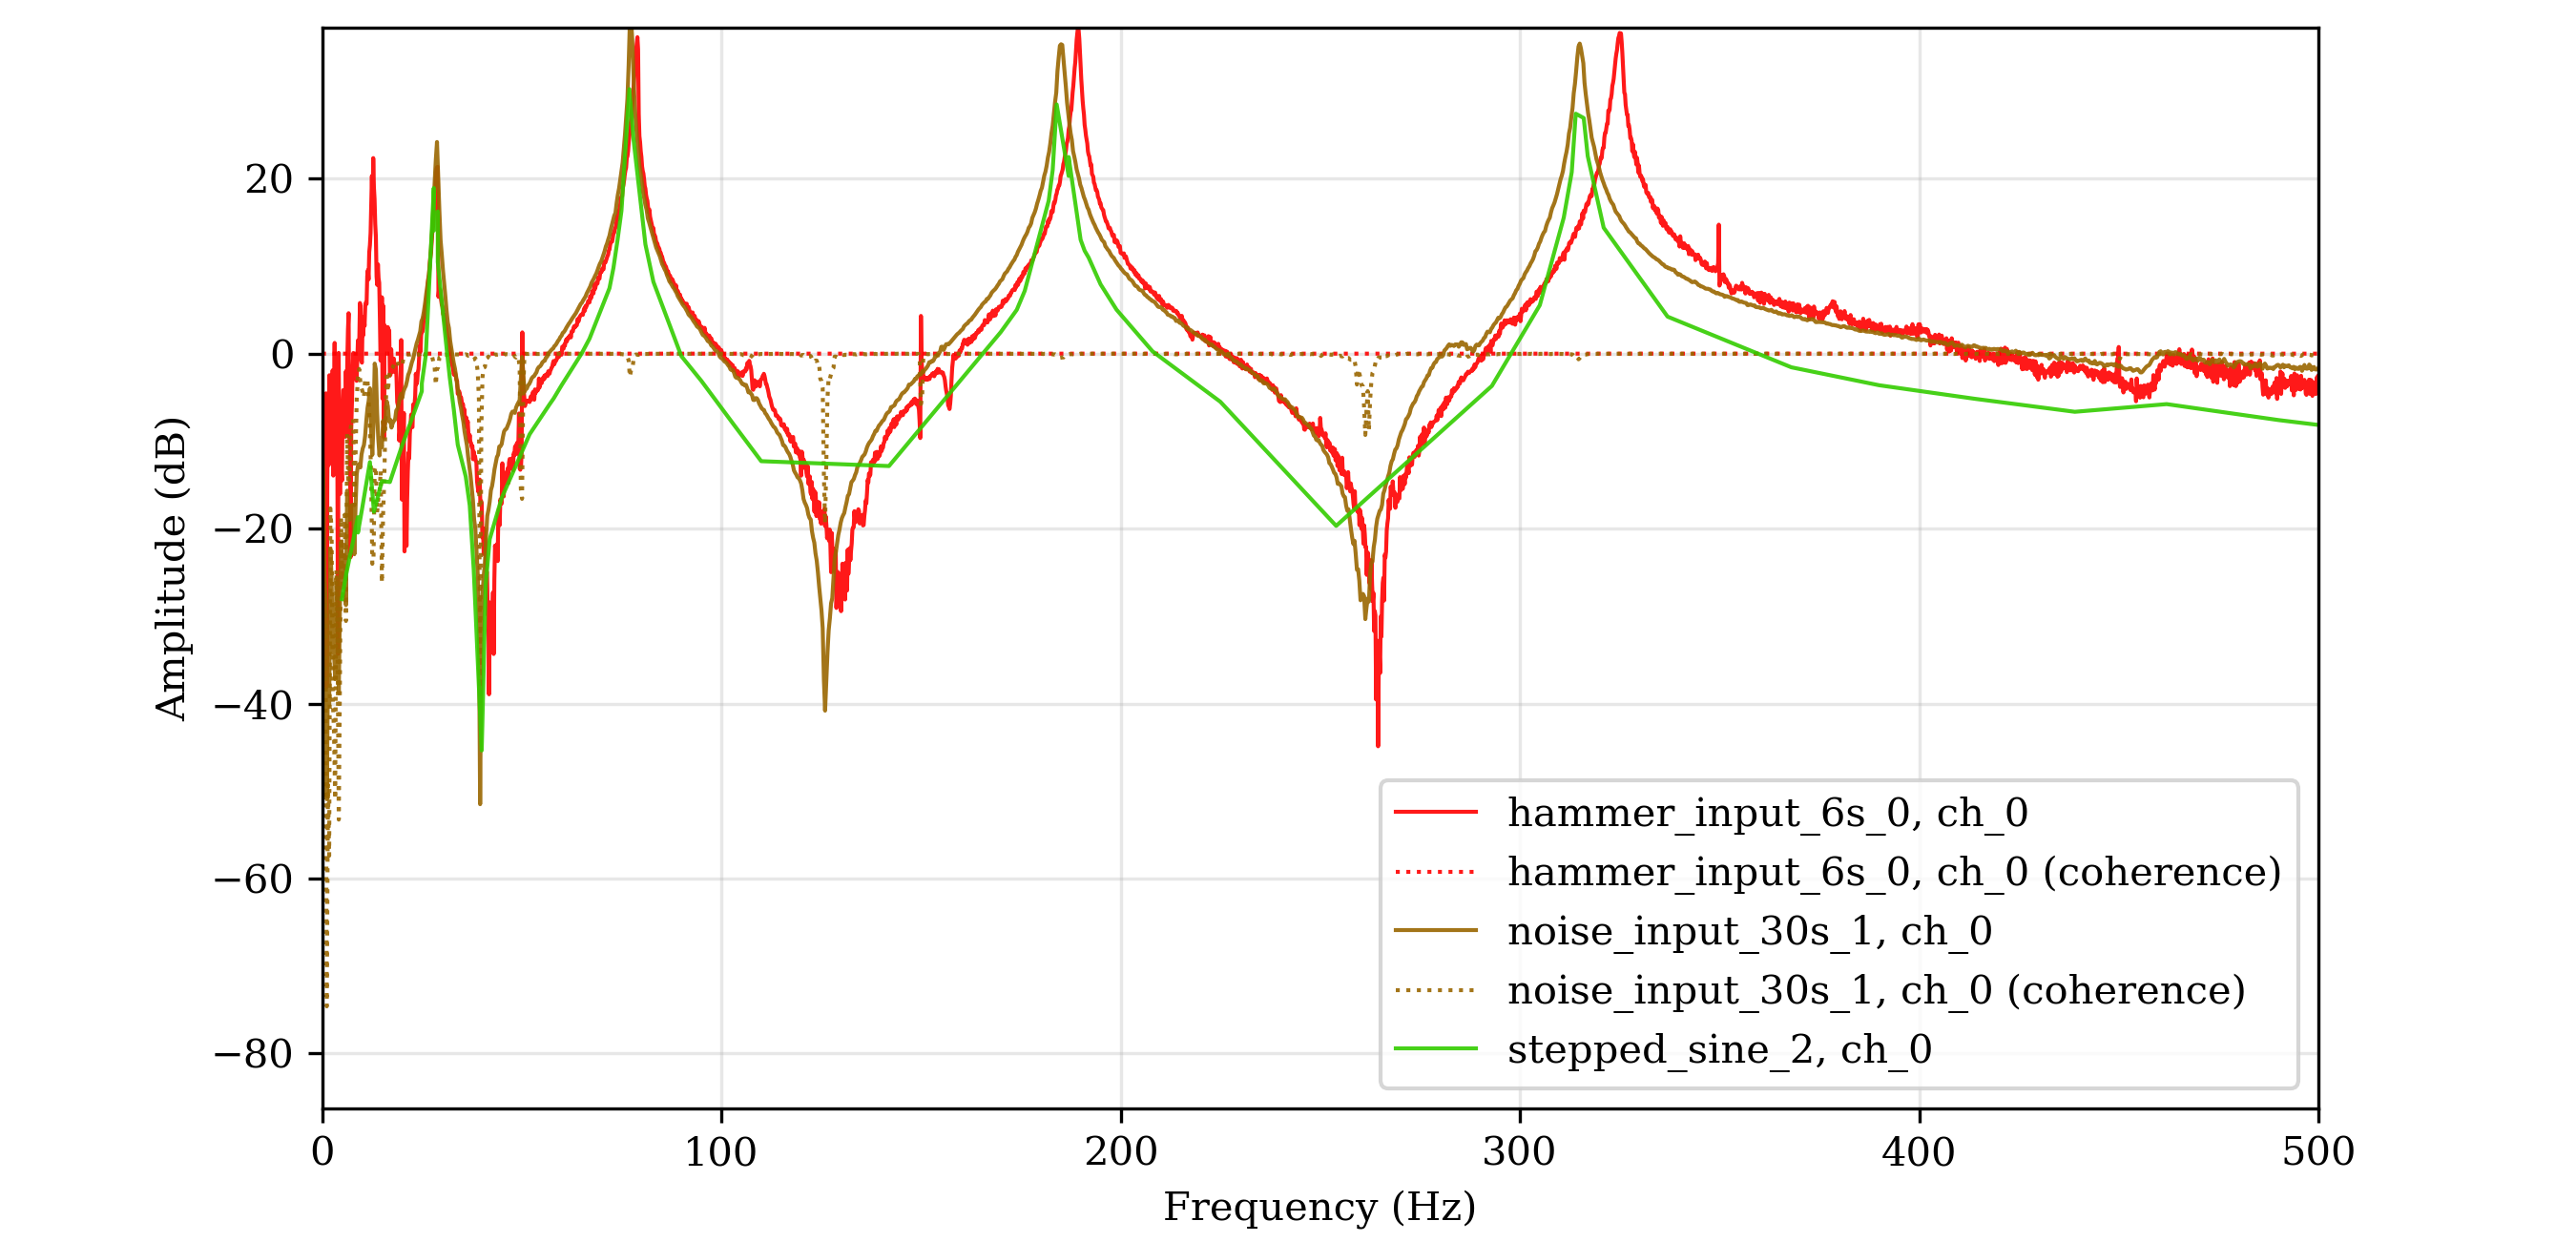
\includegraphics[width=\linewidth]{3-updatedmathcedamplitudes}
  \caption{Transfer functions for all three methods after the amplitudes have been matched}
  \label{fig:shifted}
\end{figure}


By matching the amplitude of each methods transfer function a comparison can be made between each method, this is shown in figure \ref{fig:shifted}. All three methods are consistent for frequencies 50-300Hz. At low frequencies the sine and noise method don't measure the first resonant peak. At the resonant peaks, especially the 5th peak,  the hammer method shows resonance occurring at a slightly higher frequency. This is due to a lower mass in the system as the shaker rod and magnet had been removed. Less mass gives a higher resonant frequency as $\omega_n \propto \sqrt{\frac{k}{m}}$. The measurement speed increase of the noise and hammer excitation method over a sweeped sine excitation while maintaining high accuracy makes these methods far more powerful. The addition of being able to calibrate the hammer excitation (section iv) to gain true values for acceleration is once again very useful and powerful.

\subsection{Hammer Impulse analysis}
\begin{figure*}[!htb]
    \centering
    \begin{subfigure}[t]{0.5\textwidth}
        \centering
        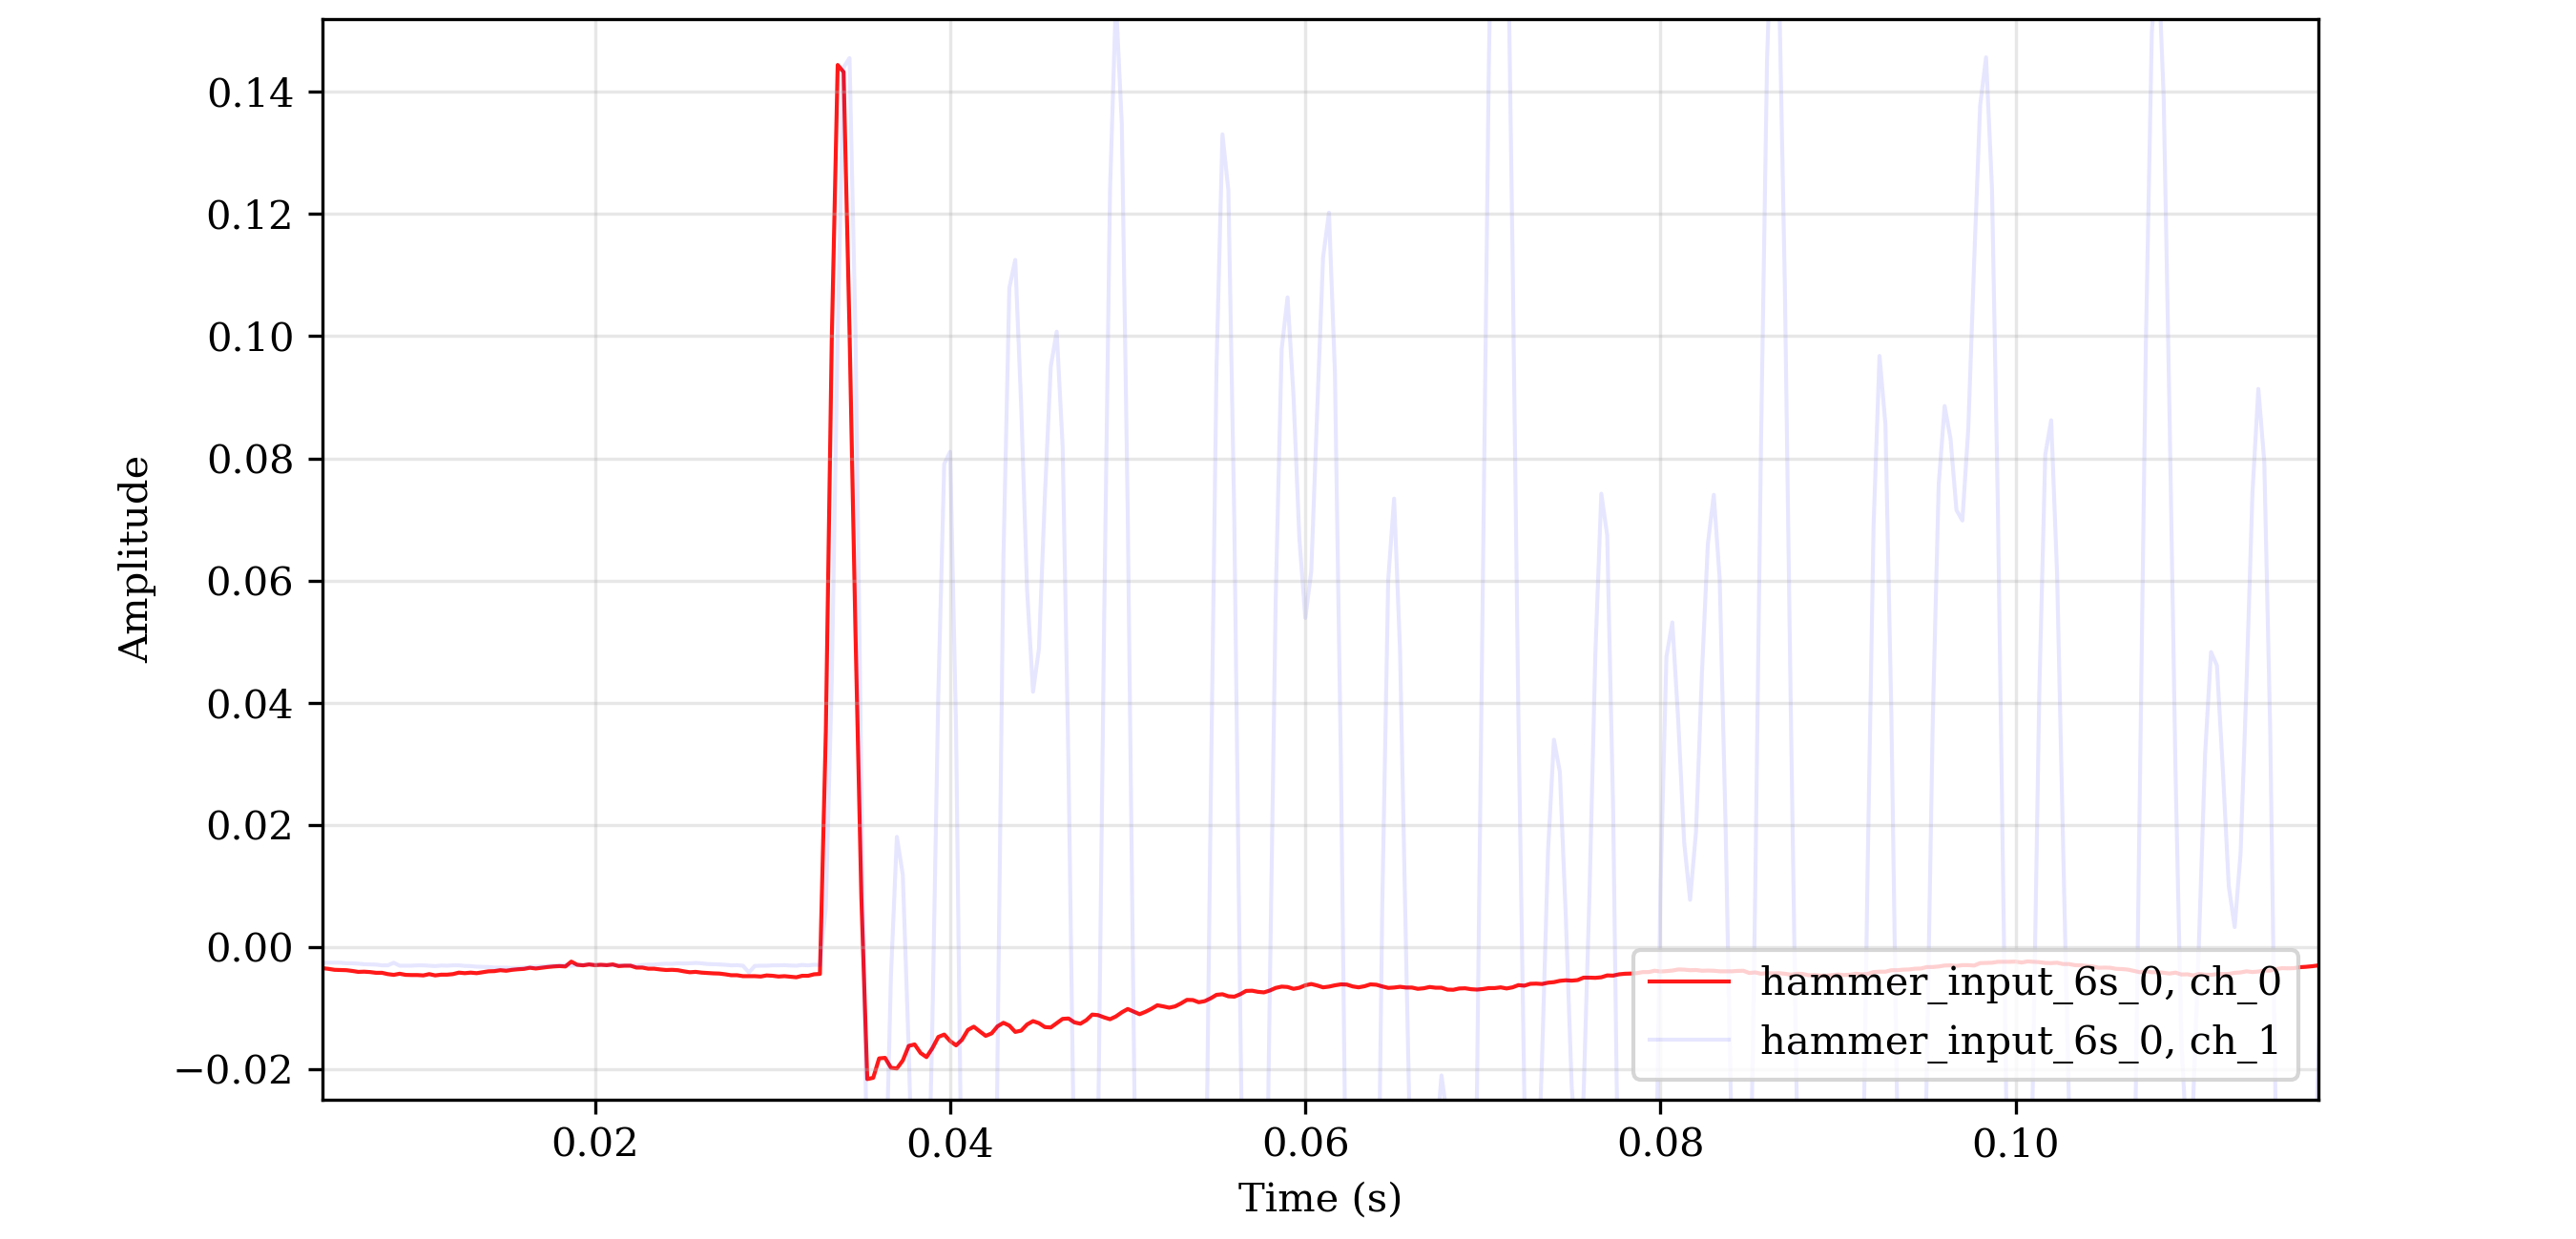
\includegraphics[height=1.55in]{3-updatedhammershape}
        \caption{Hammer Impulse Shape}
    \end{subfigure}%
    ~ 
    \begin{subfigure}[t]{0.5\textwidth}
        \centering
        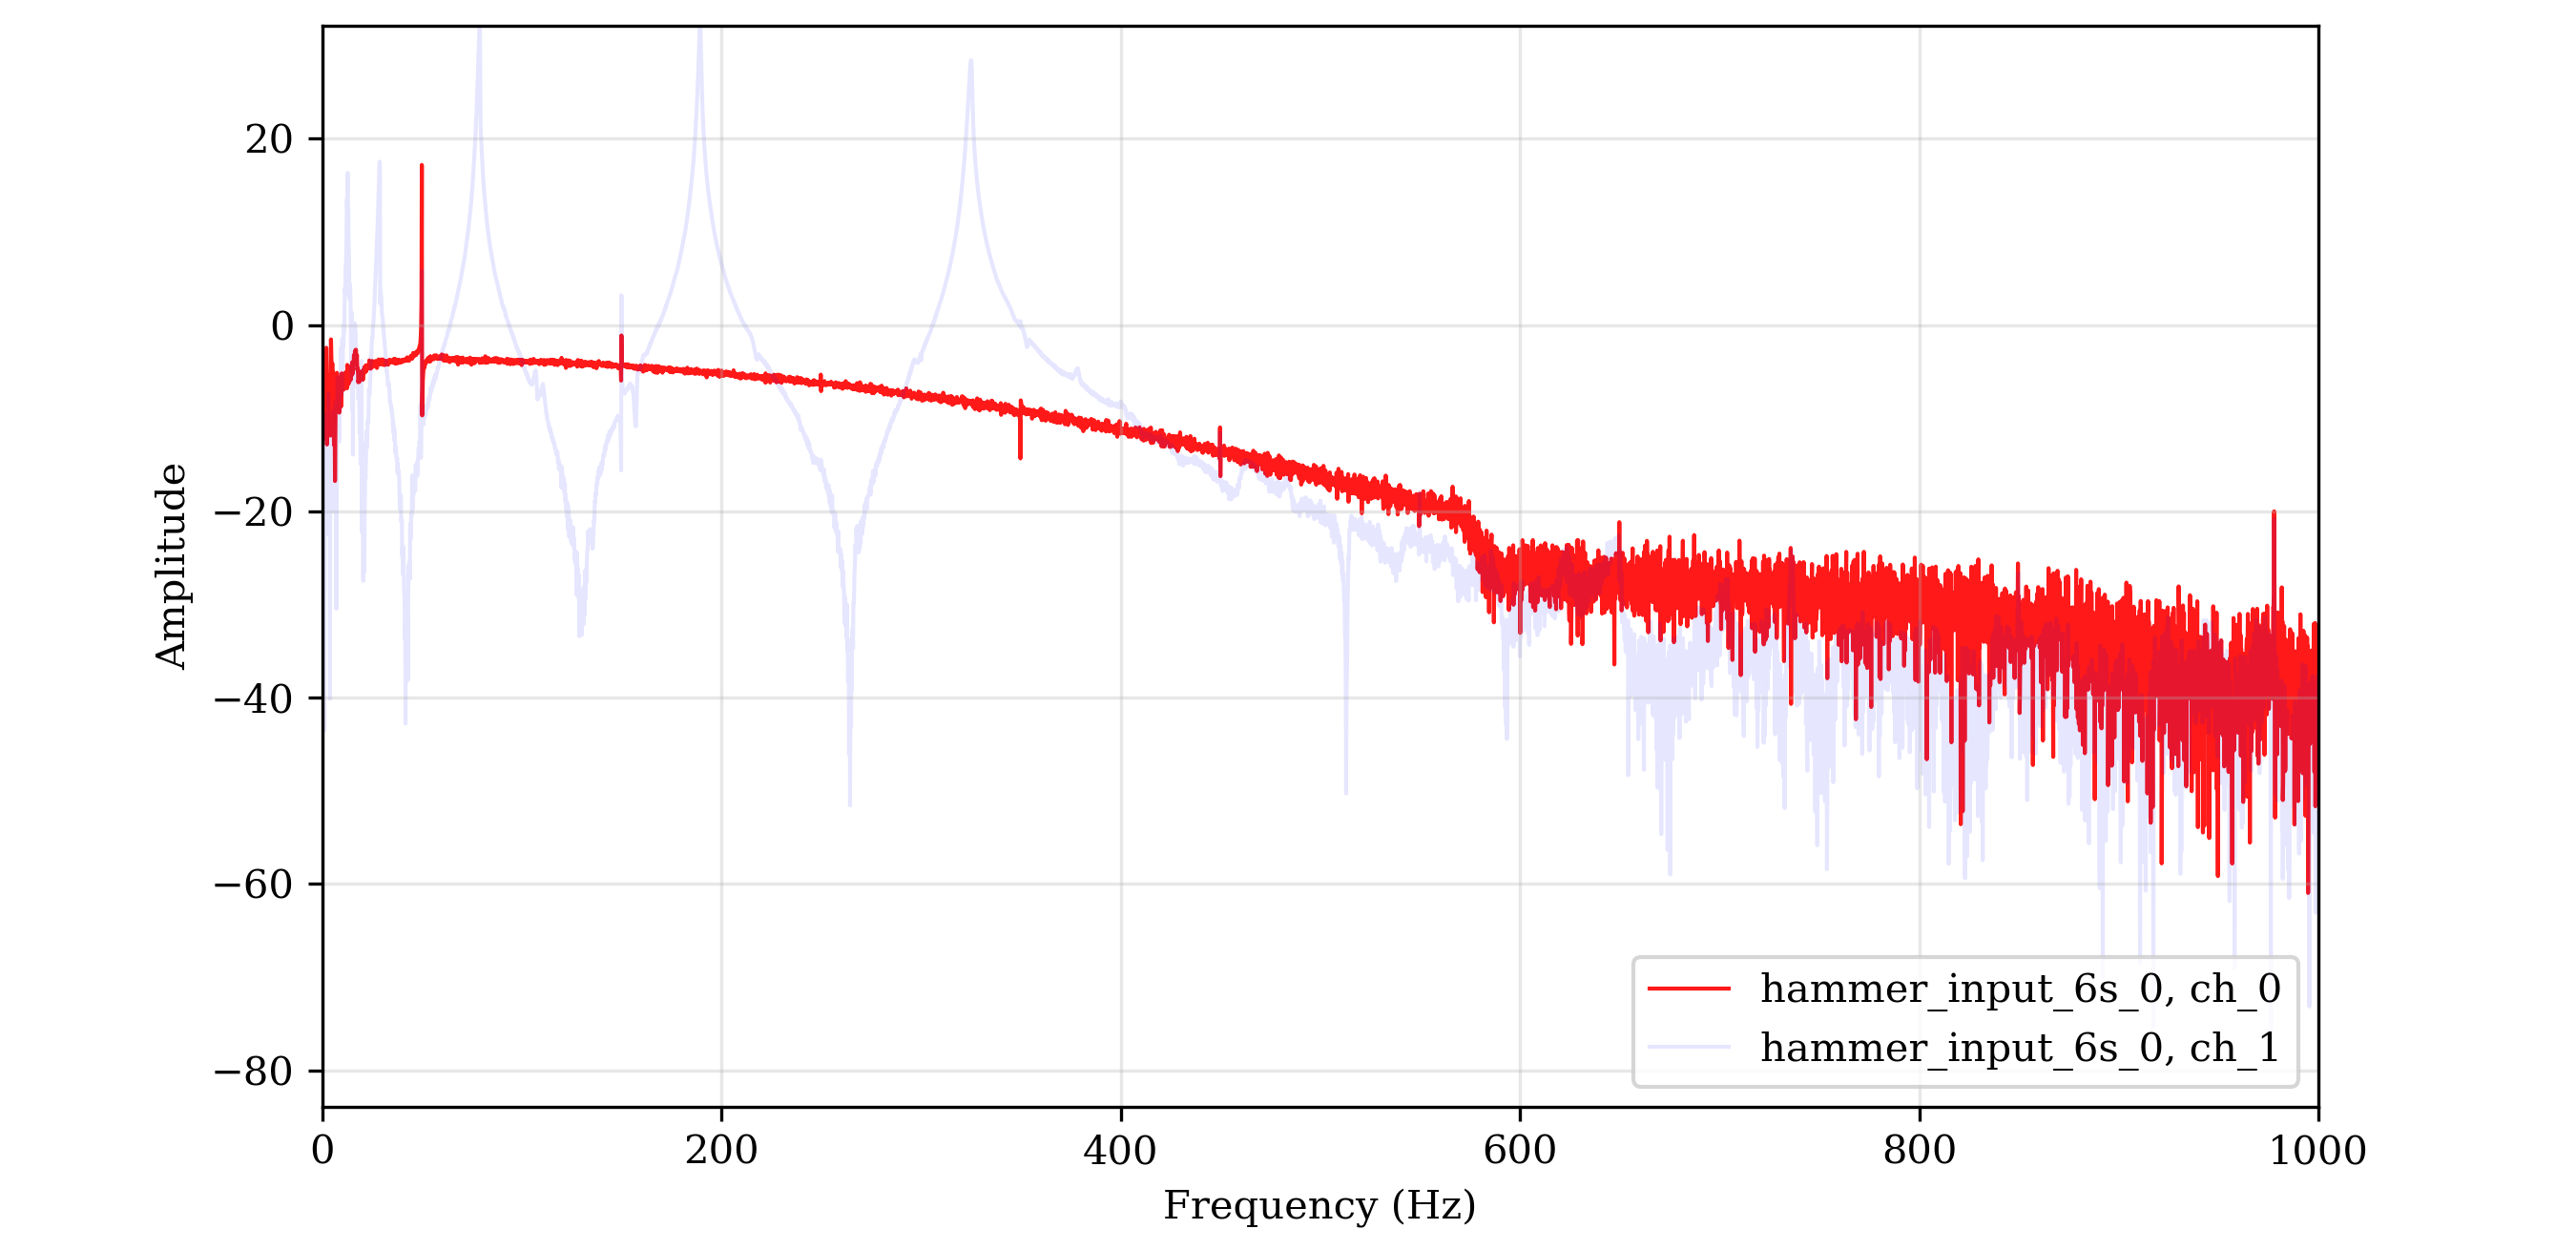
\includegraphics[height=1.55in]{3-updatedffthammer}
        \caption{FFT of Impulse}
    \end{subfigure}
    \caption{Hammer input in the time and frequency domain}
    \label{fig:impulse}
\end{figure*}

An ideal impulse $\delta(t)$ would input every frequency at constant magnitude as the Fourier transform of this is: $\mathcal{F}(\delta(t))=1$. This would require an instantaneous force input into the structure which isn't physically possible and would damage the structure if it was. Instead the impulse input is similar to figure \ref{fig:impulse}, which shows a finite time triangular pulse or half cosine, followed by overshoot and a oscillatory decay back to the datum force level. 
The shape of the input arises due to the following factors:
\begin{itemize}
\item Non zero input before and after a hit - caused by sensor and electrical noise in addition to slight movements of the hammer compressing the piezoelectric sensor.
\item Finite pulse time - caused by finite contact time in the impact. The rubber tip acts like a spring and contracts during the hit which creates the maximum force, then extends and the force profile lowers again.
\item Overshoot after the pulse - the piezoelectric crystal can't measure a constant DC force, this means it acts as a high pass filter with slow time constant. This causes a 'negative' force or extension to be measured so that the normalised force at DC =0. The slow time constant causes the slow decay back to zero force.
\item Oscillations or ringing - the hammer signal is filtered with a low pass filter to avoid aliasing effects when taking Fourier transforms. This means the smooth decaying shape isn't recorded as higher frequencies are missing. Therefore causing the observed ringing behaviour.
\end{itemize}

Treating the impulse as a half-cosine wave of width 'T', height 'a' and taking Fourier transforms gives equation \ref{eq:cosfourier}.

\begin{equation}
\mathcal{F}(\omega)= \frac{aT}{2}(sinc\frac{\omega T-\pi}{2} + sinc \frac{\omega T+\pi}{2})
\label{eq:cosfourier}
\end{equation}


\begin{figure}[!htb]
  \centering
    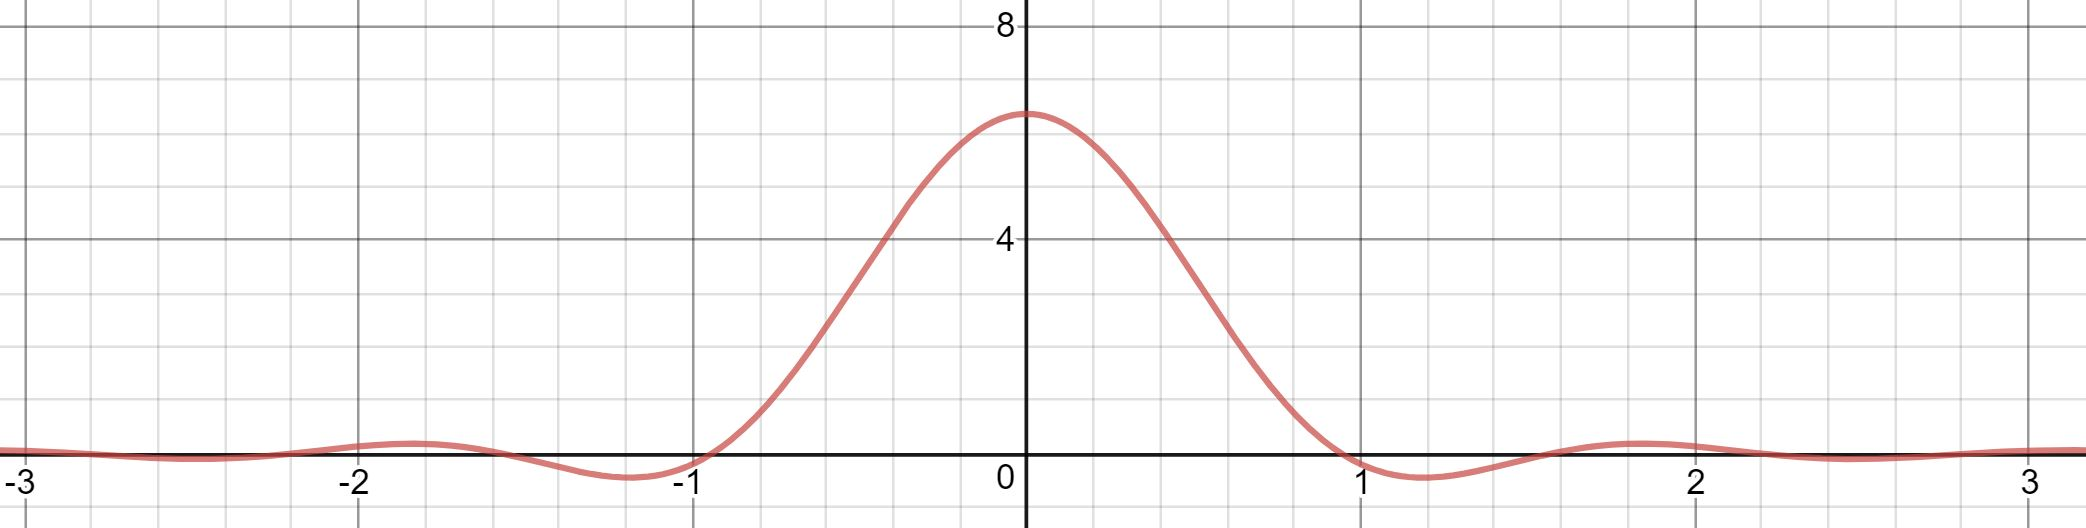
\includegraphics[width=\linewidth]{sinc}
  \caption{$\mathcal{F}(\omega)$ as in equation \ref{eq:cosfourier} with a=1, T=10.}
  \label{fig:sinc}
\end{figure}

Figure \ref{fig:sinc} shows that the majority of the frequencies occur within the first lobe of the function. This occurs when $sin\frac{\omega T-\pi}{2}=0=sin\frac{\omega T+\pi}{2}$. Therefore, $\frac{\omega T-\pi}{2}=\pi n =\frac{\omega T+\pi}{2}$. This gives the first zero at $\omega = \frac{3\pi}{T}$, as it can't be $\frac{\pi}{T}$ due to sinc(0) being non zero. The bandwidth can then be approximated as $2\omega = \frac{6\pi}{T}$. In our impulse T=2.5ms giving a bandwidth of approximately 1200Hz. This value is larger than shown in figure \ref{fig:impulse}, however this is likely the low pass filter incorporated in the measurement equipment attenuating frequencies above 600Hz, hence causing the low amplitude noisy response above this value.
\newline

The range of frequencies of interest must be present in the bandwidth of our pulse. This corresponds to making the pulse duration short enough to involve these frequencies. A short pulse can be achieved in two ways. Firstly a low hammer mass means a lower force and time is required to reverse the hammer direction, this factor is typically fixed or adjusted to ensure enough energy is input to excite all modes of interest. Having a large stiffness on the tip means the force required to change directions happens after less compression and therefore less time. Rubber has a stiffness that allows for suitable pulse duration for observing 0-500Hz. A material with a larger stiffness (eg steel) is not used as this could damage the structure and the sensitivity to noise from random pressure on the tip is greater. Therefore a rubber tip gives a happy medium for generating the required frequencies with decent resilience to noise.
%--------------------------------------------------------------]
\subsection{Calibration}
\begin{figure}[h]
  \centering
    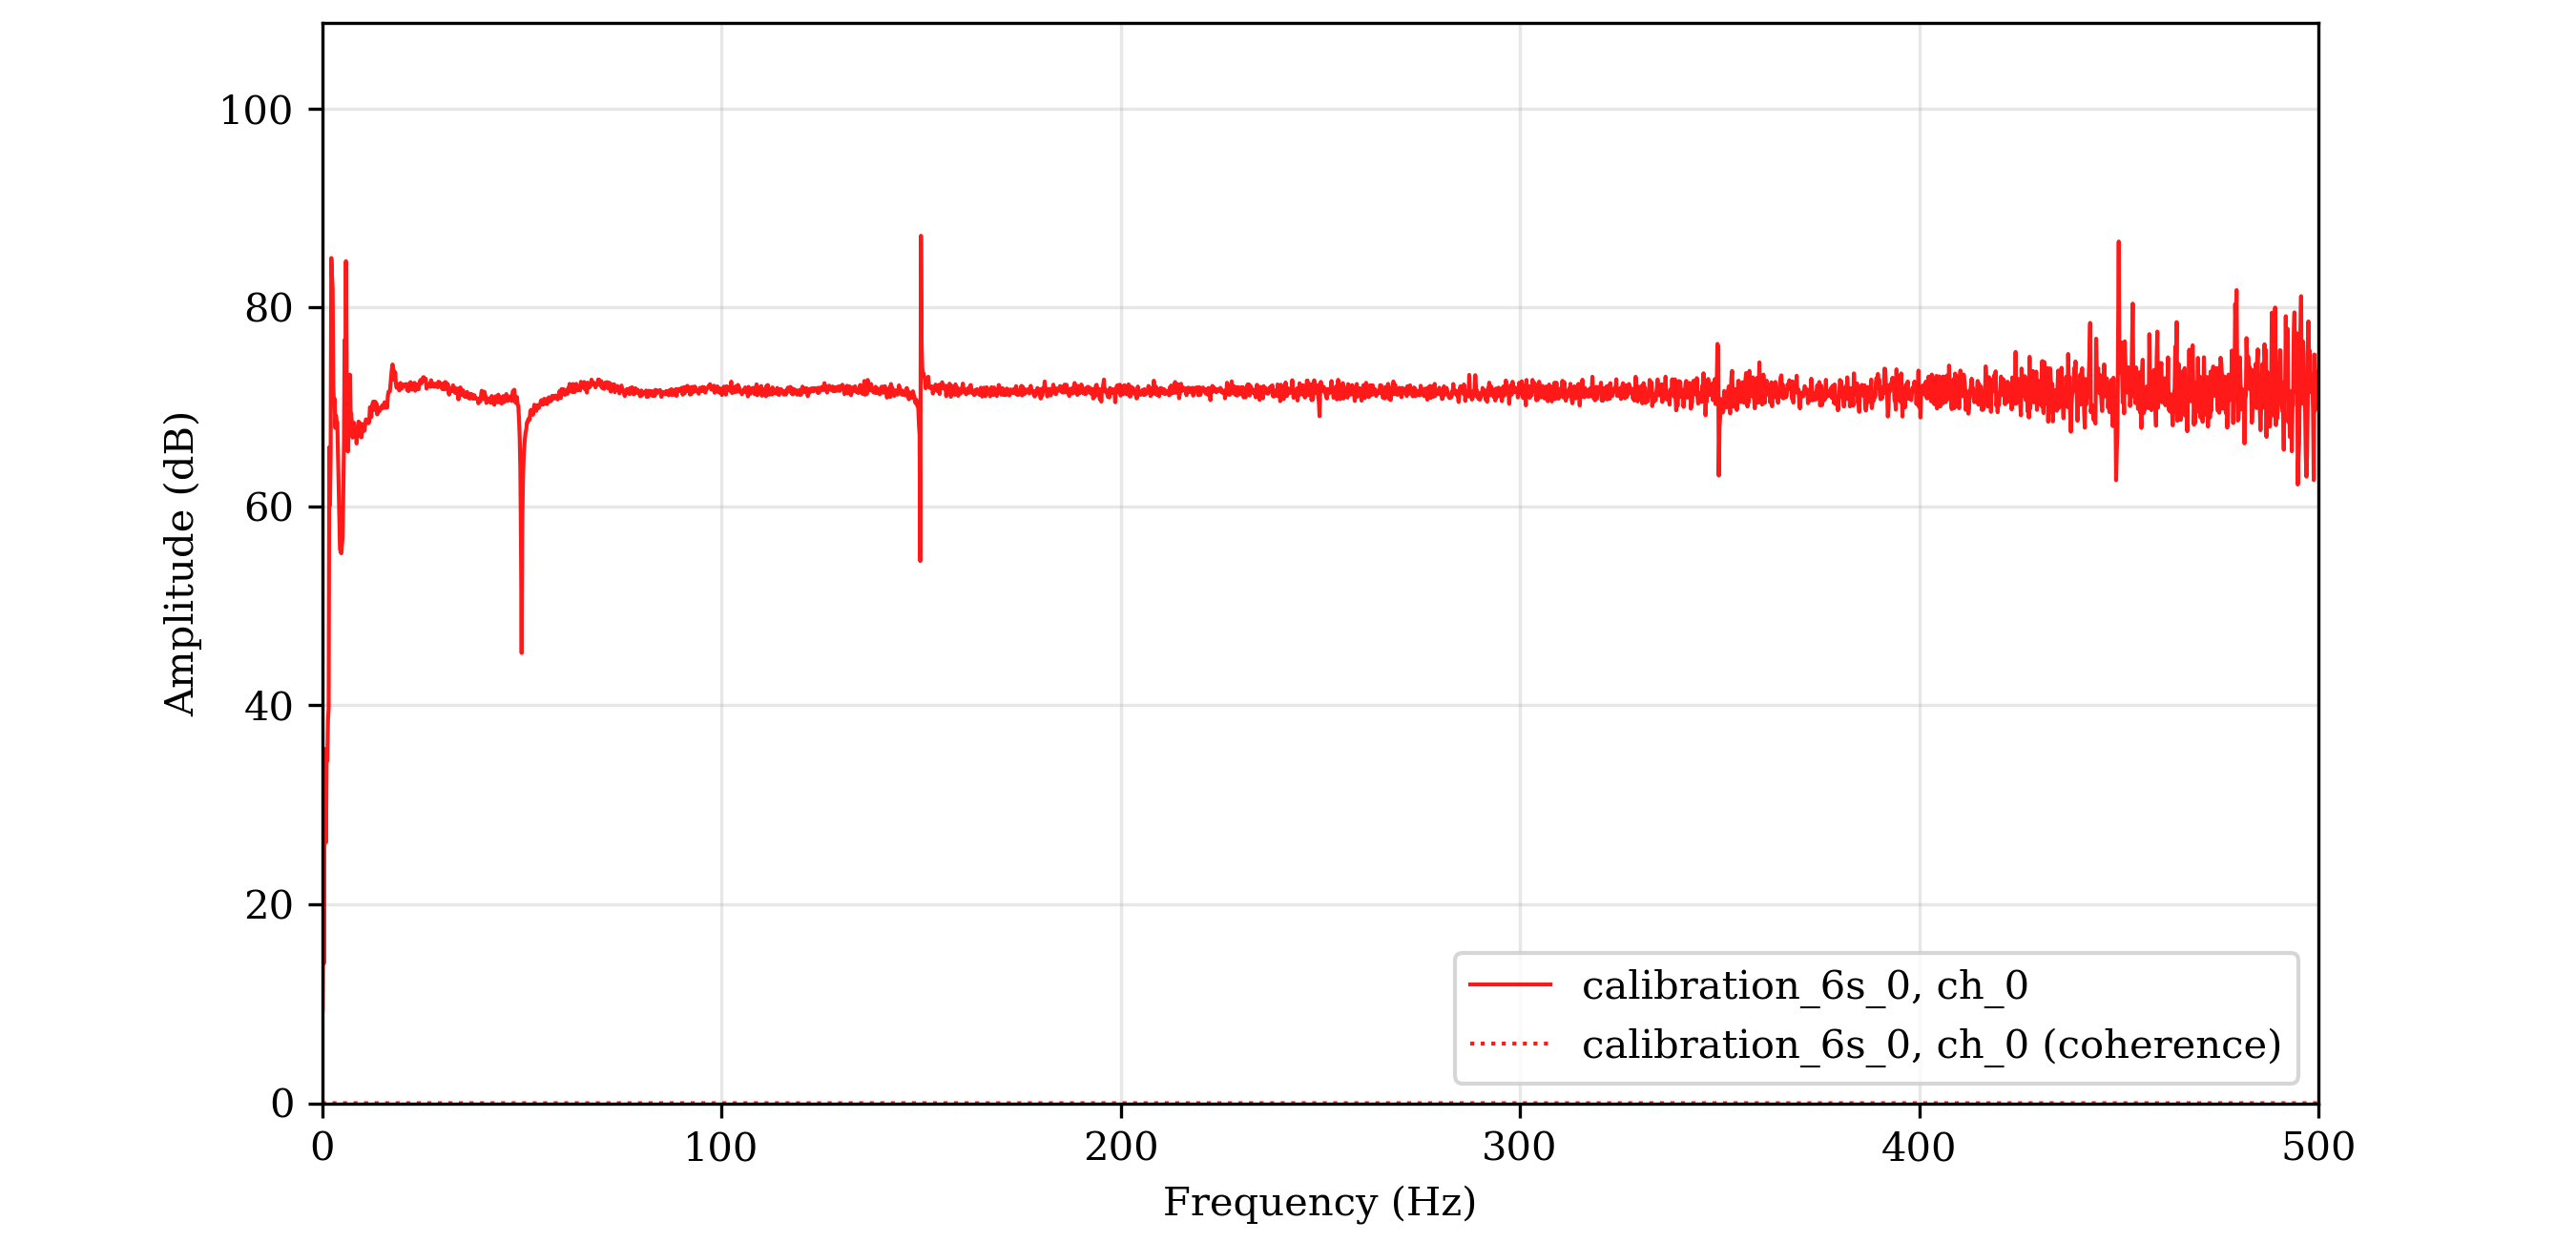
\includegraphics[width=\linewidth]{4-calibrationhit}
  \caption{Transfer function relating to acceleration of the hanging mass due to a hammer impulse}
  \label{fig:calhit}
\end{figure}

The hammer force readings can be calibrated by measuring on a system with known transfer function to obtain true accelerations. The system chosen is a suspended mass. The transfer function is shown in equation \ref{TF}.


\begin{equation}
\label{TF}
\frac{a(s)}{F(s)}=m = \frac{1}{0.369}=2.71
\end{equation}

This is a constant transfer function between acceleration and force and is shown experimentally in figure \ref{fig:calhit} as an almost constant line at 72dB across frequencies (except for peaks at 50Hz intervals from the mains). This corresponds to a linear value of 3981 which must match the true value of $\frac{a}{F}=2.71$. This gives a calibration factor of $\frac{2.71}{3981}=6.6x10^{-4}$.  

%--------------------------------------------------------------
\subsection{Comparison of calibrated Responses}
\begin{figure}[!htb]
  \centering
    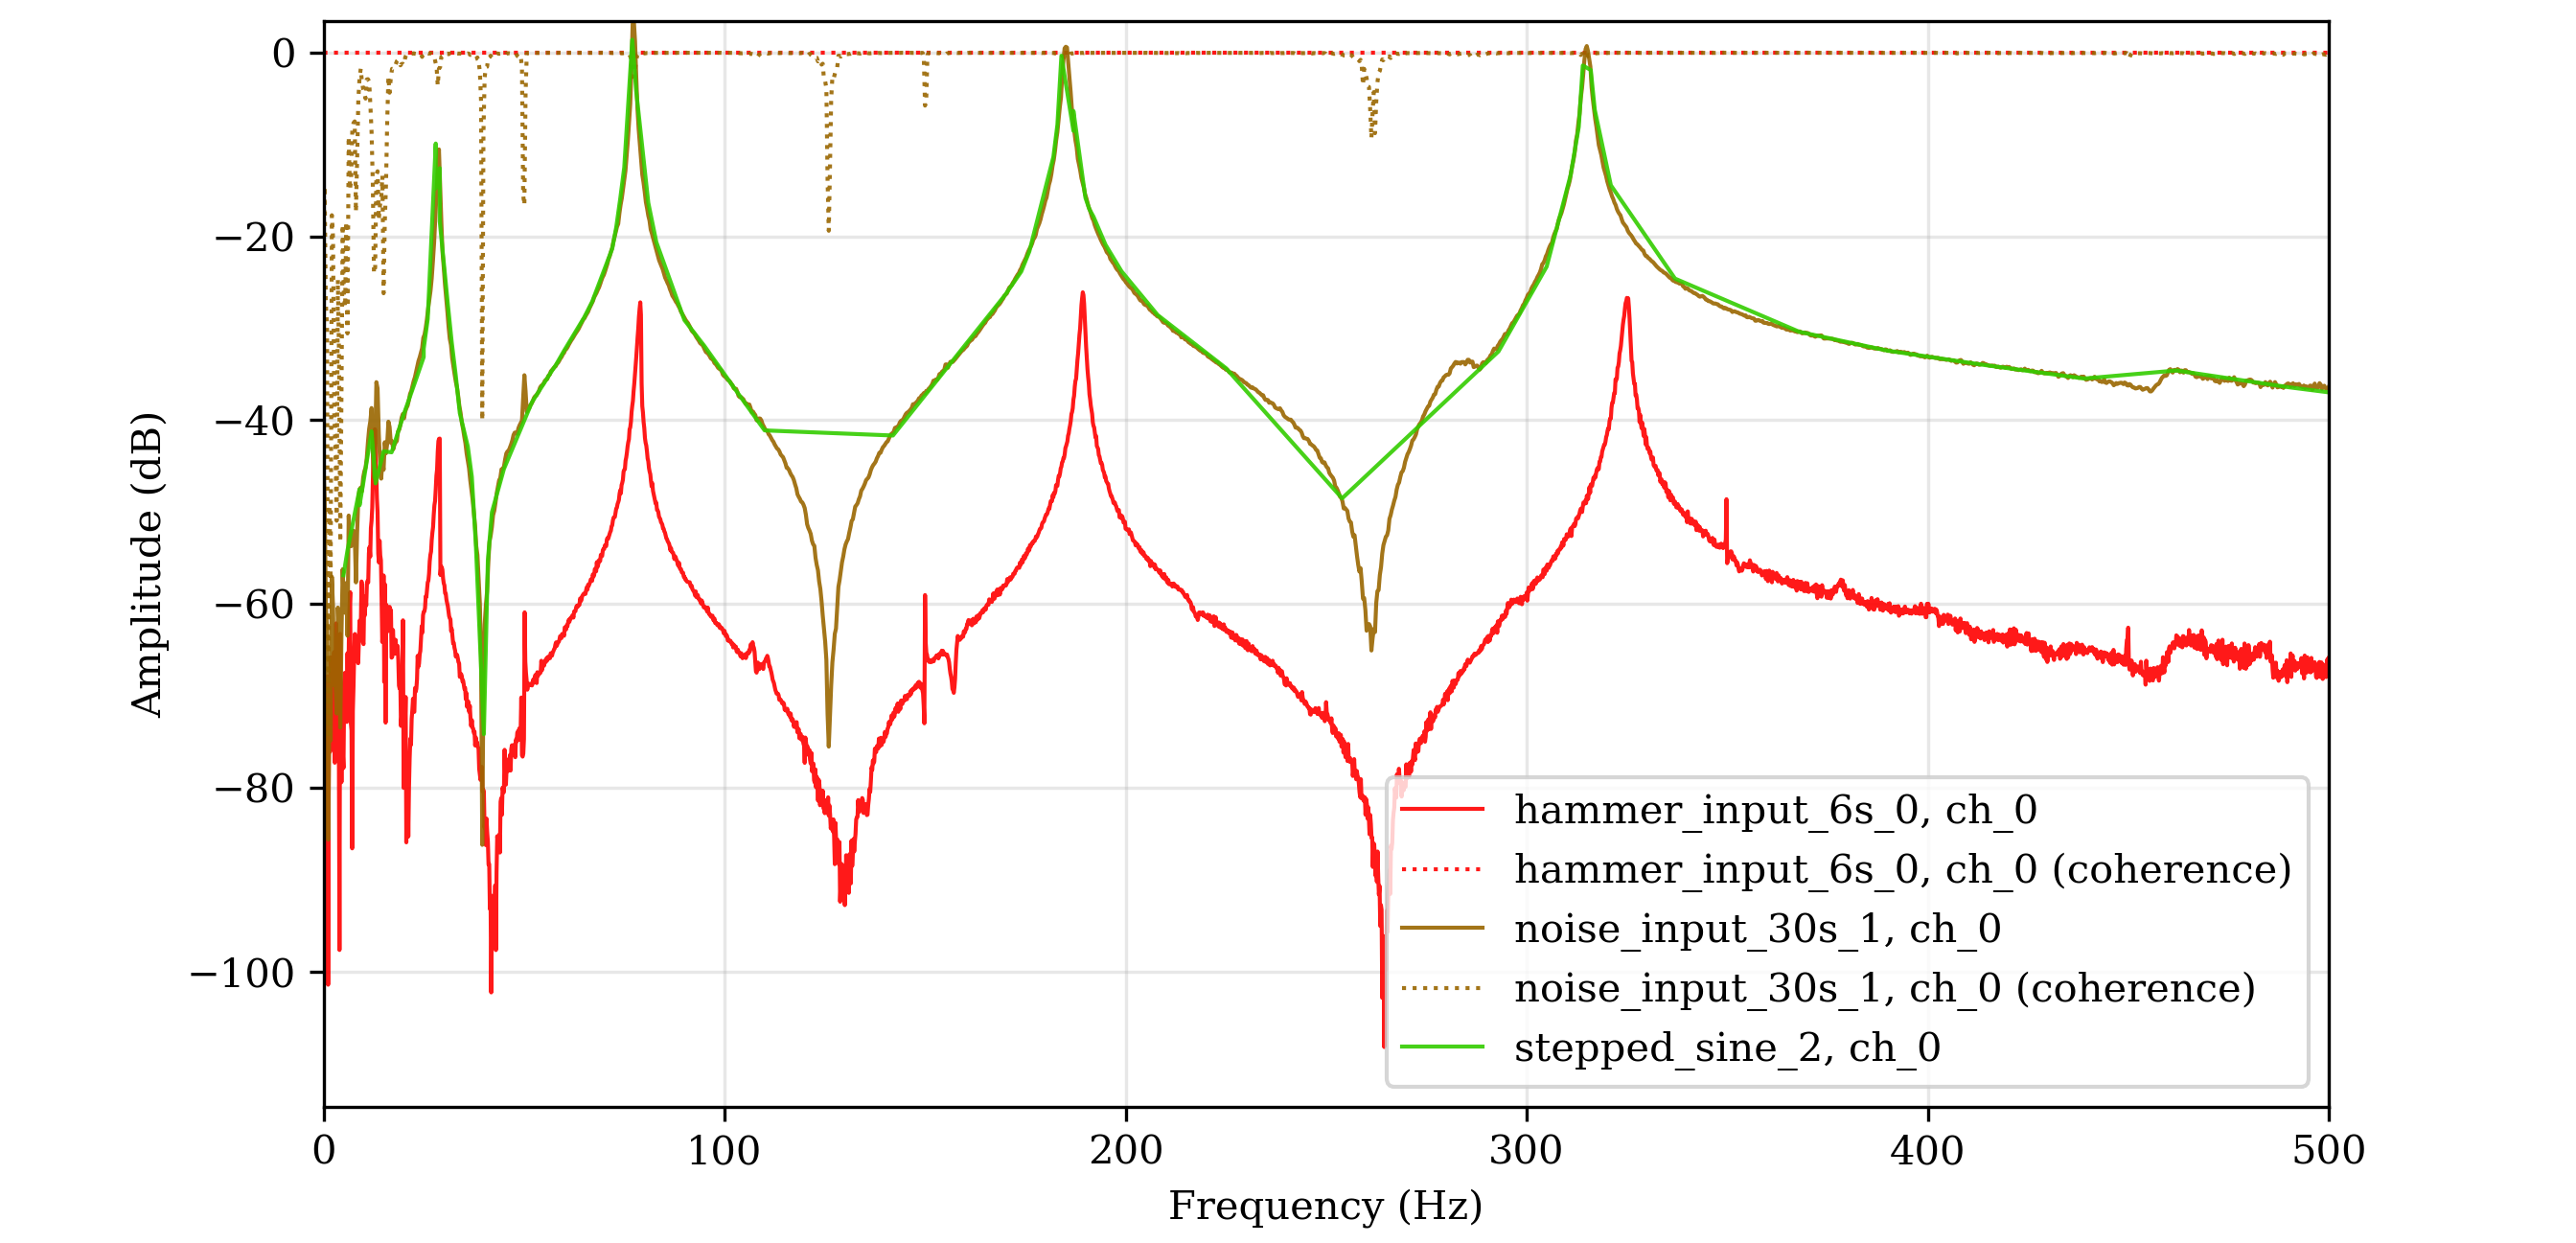
\includegraphics[width=\linewidth]{5-updatedcalibrationbefore}
  \caption{Transfer functions for each measurement technique before calibration }
  \label{fig:3b}
\end{figure}
By using the calibration factor calculated in section iv the hammer excitation transfer function can be rescaled to represent true accelerations. The other techniques can then have their amplitudes matched to this calibrated hammer transfer function. This transforms figure \ref{fig:3b} into figure \ref{fig:3a}. From this you can see that resonances reach a peak ratio between a and F of approximately -25dB = 0.056. The lower and higher frequencies aren't shown as they are too noisy to be matched accurately between methods.
\begin{figure}[!htb]
  \centering
    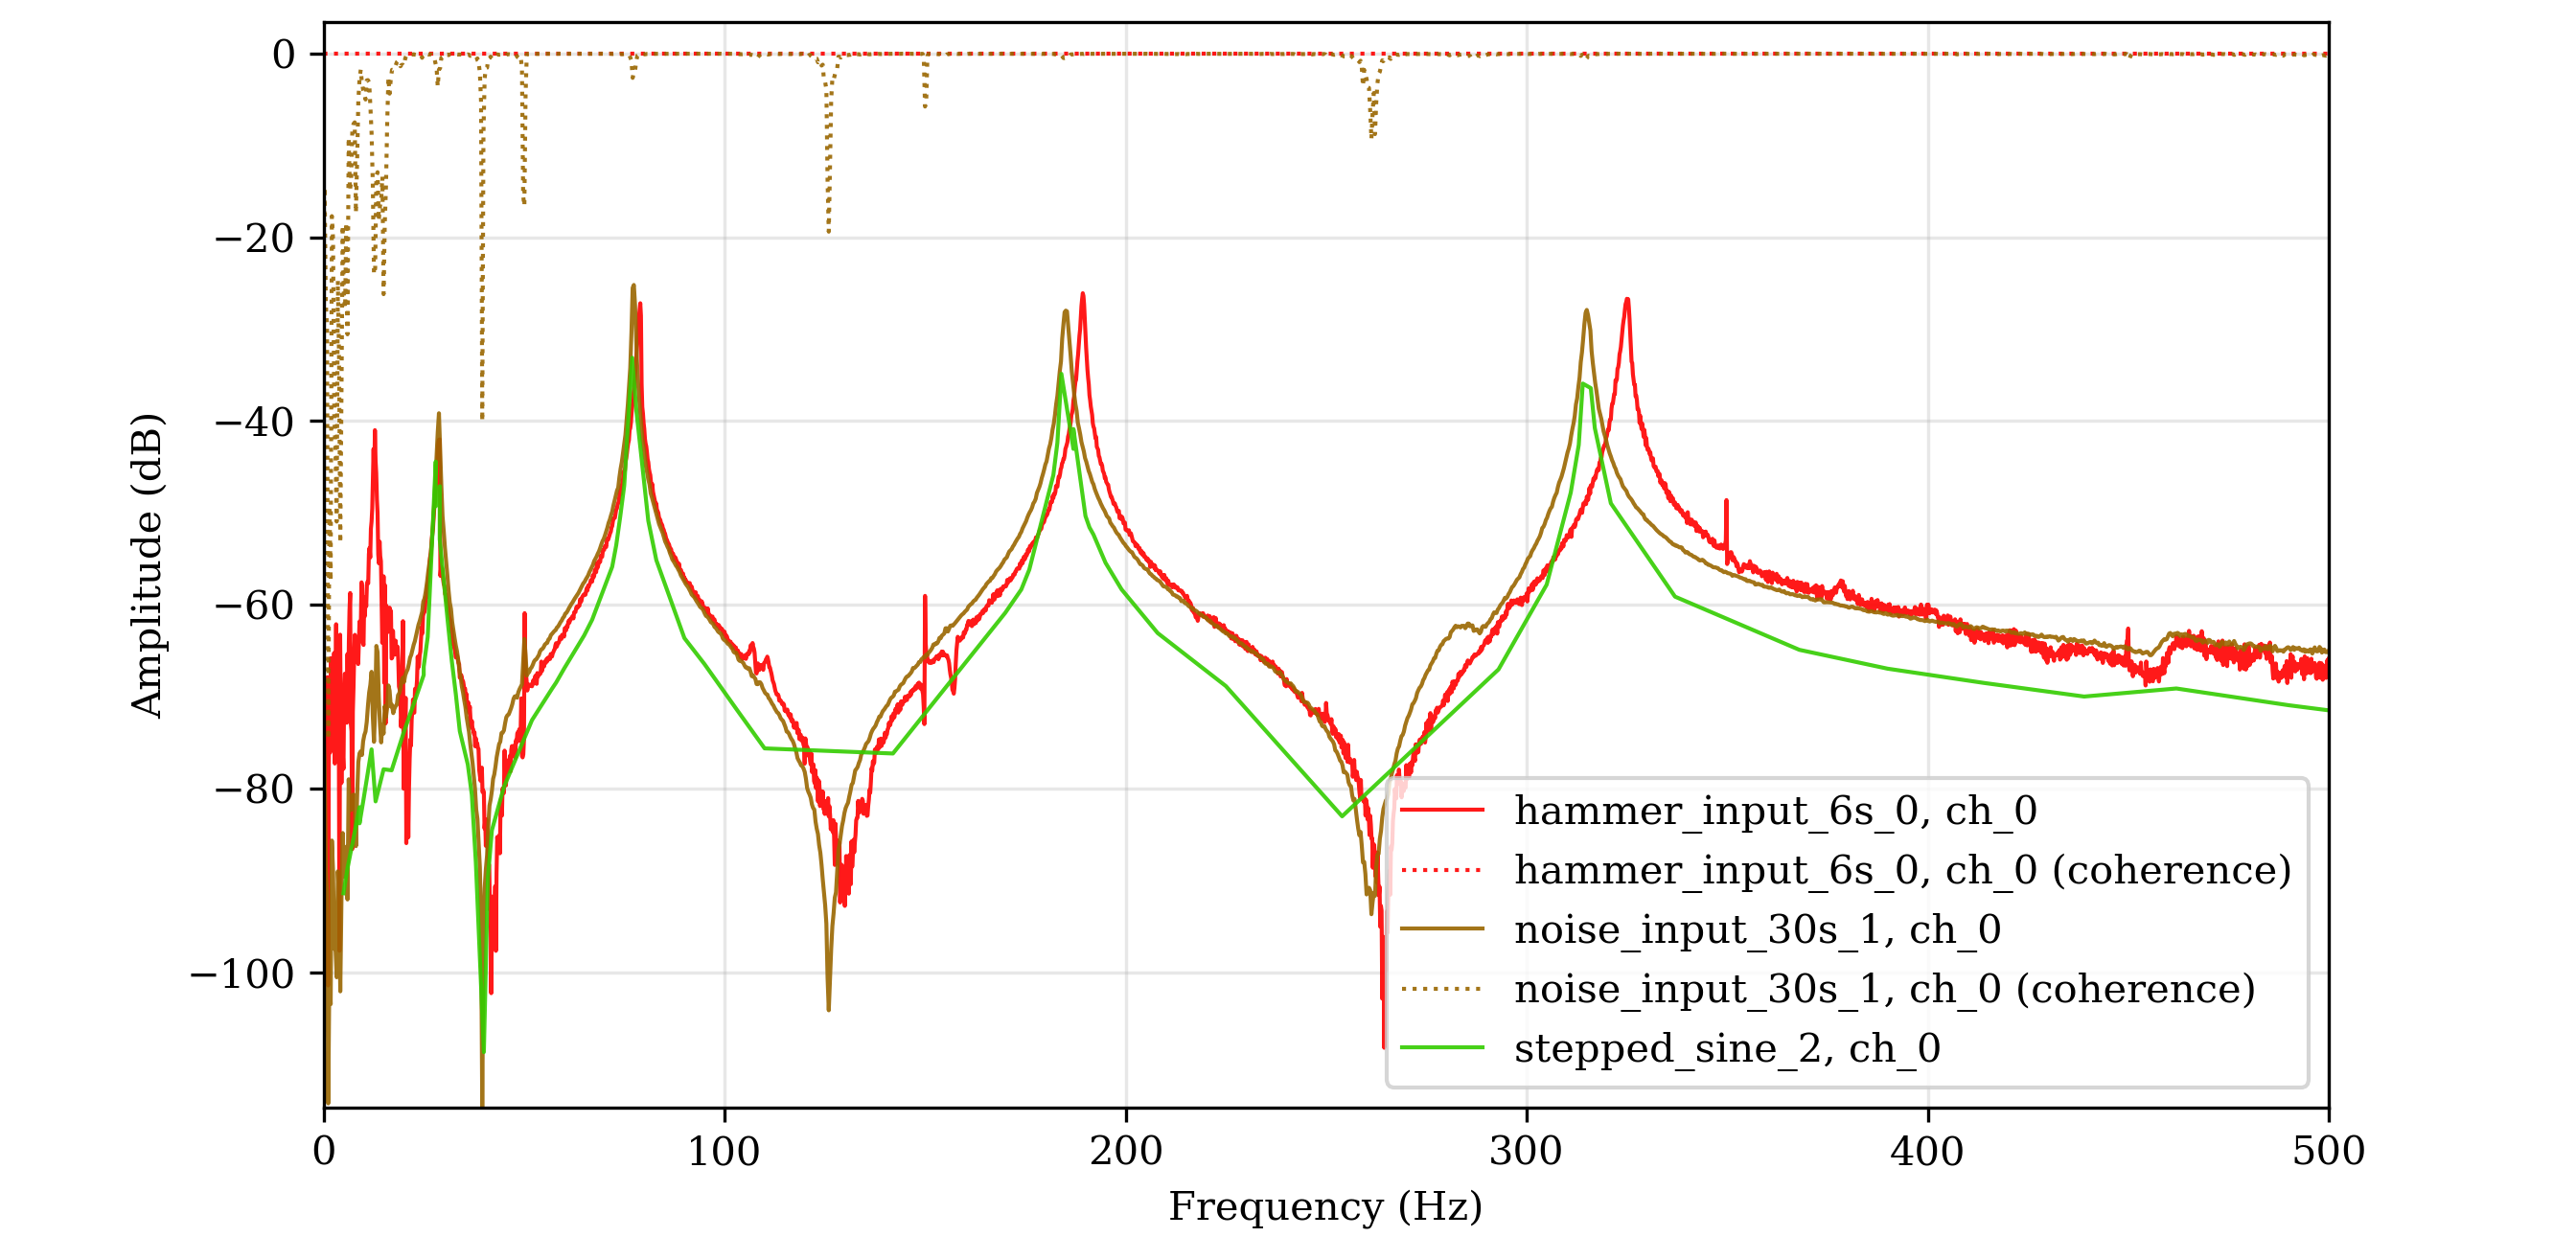
\includegraphics[width=\linewidth]{5-updatedcalibrationafter}
  \caption{Transfer functions for each measurement technique after calibration }
  \label{fig:3a}
\end{figure}



%--------------------------------------------------------------
\subsection{Coupled System Response}
\begin{figure}[!htb]
  \centering
    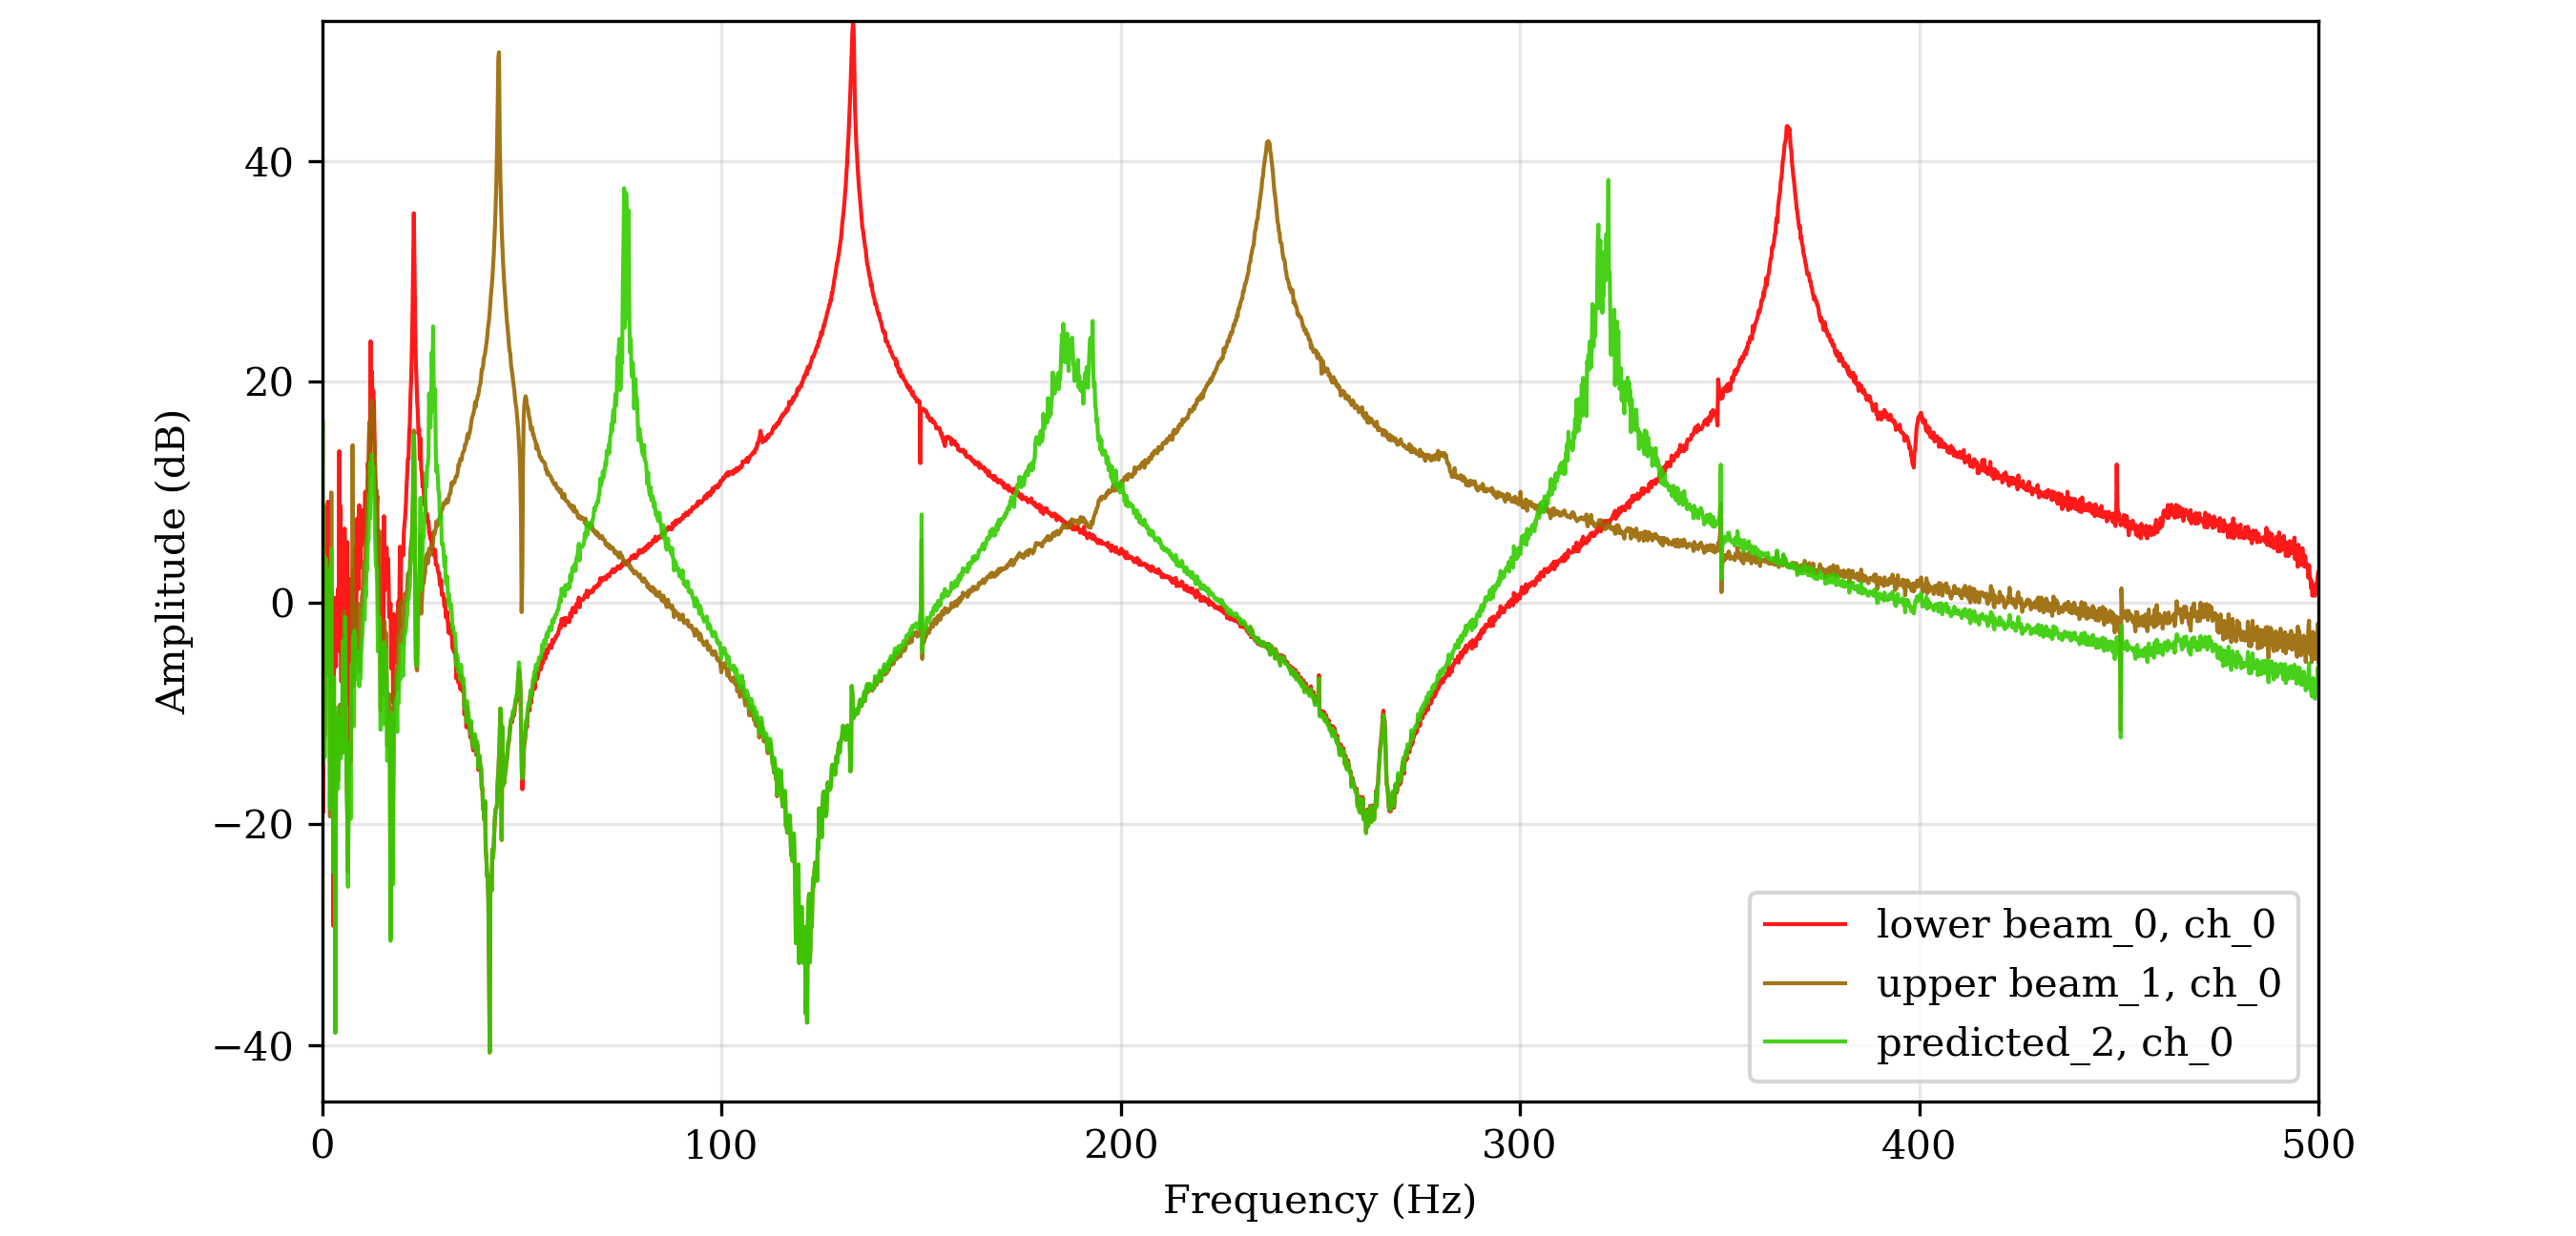
\includegraphics[width=\linewidth]{6-coupled}
  \caption{Transfer functions using a hammer on the two beams uncoupled, with a prediction for the coupled behaviour }
  \label{fig:uncoupled}
\end{figure}

When the couple connecting the two cantilever beams is removed you can measure the response of each beam independently then a prediction of the coupled response can be made. This prediction uses the fact that when coupled the attachment points have the same velocity and amplitude see equation \ref{coupledeq}. Figure \ref{fig:uncoupled} shows these transfer functions. At low frequencies there is still lots of noise however the 1st resonant is just visible. The upper and lower beams alternate resonant peaks, with the coupled prediction peak residing at the frequency of intersection between the two responses. This location matches with the theory as poles occur when the denominator = 0 which is when the magnitude of $Y_{top}=Y_{bot}$ and the two are in anti-phase. The anti-resonances appear in the same location for the predicted plot and each beam individually, this one again agrees with theory. Anti-resonances reside between each resonant peak, this is expected as measuring and exciting from the same point causes $u_j^{(n)}u_k^{(n)}$ to always be positive and therefore cause anti-resonance. The definition of the predicted peaks is low and more noise is present. This loss of clarity is due to the lower quality measurement (lower SNR) dominating when predicting the transfer function using equation \ref{coupledeq}. The smaller response in the sum with subsequently higher SNR dominates.  The only resonant peak that is shared between the cantilevers is the lowest one. This further shows that this vibration mode involves the whole structure bouncing on the rubber supports and therefore can be excited by applying an external force to either beam.
\begin{figure}[!htb]
  \centering
    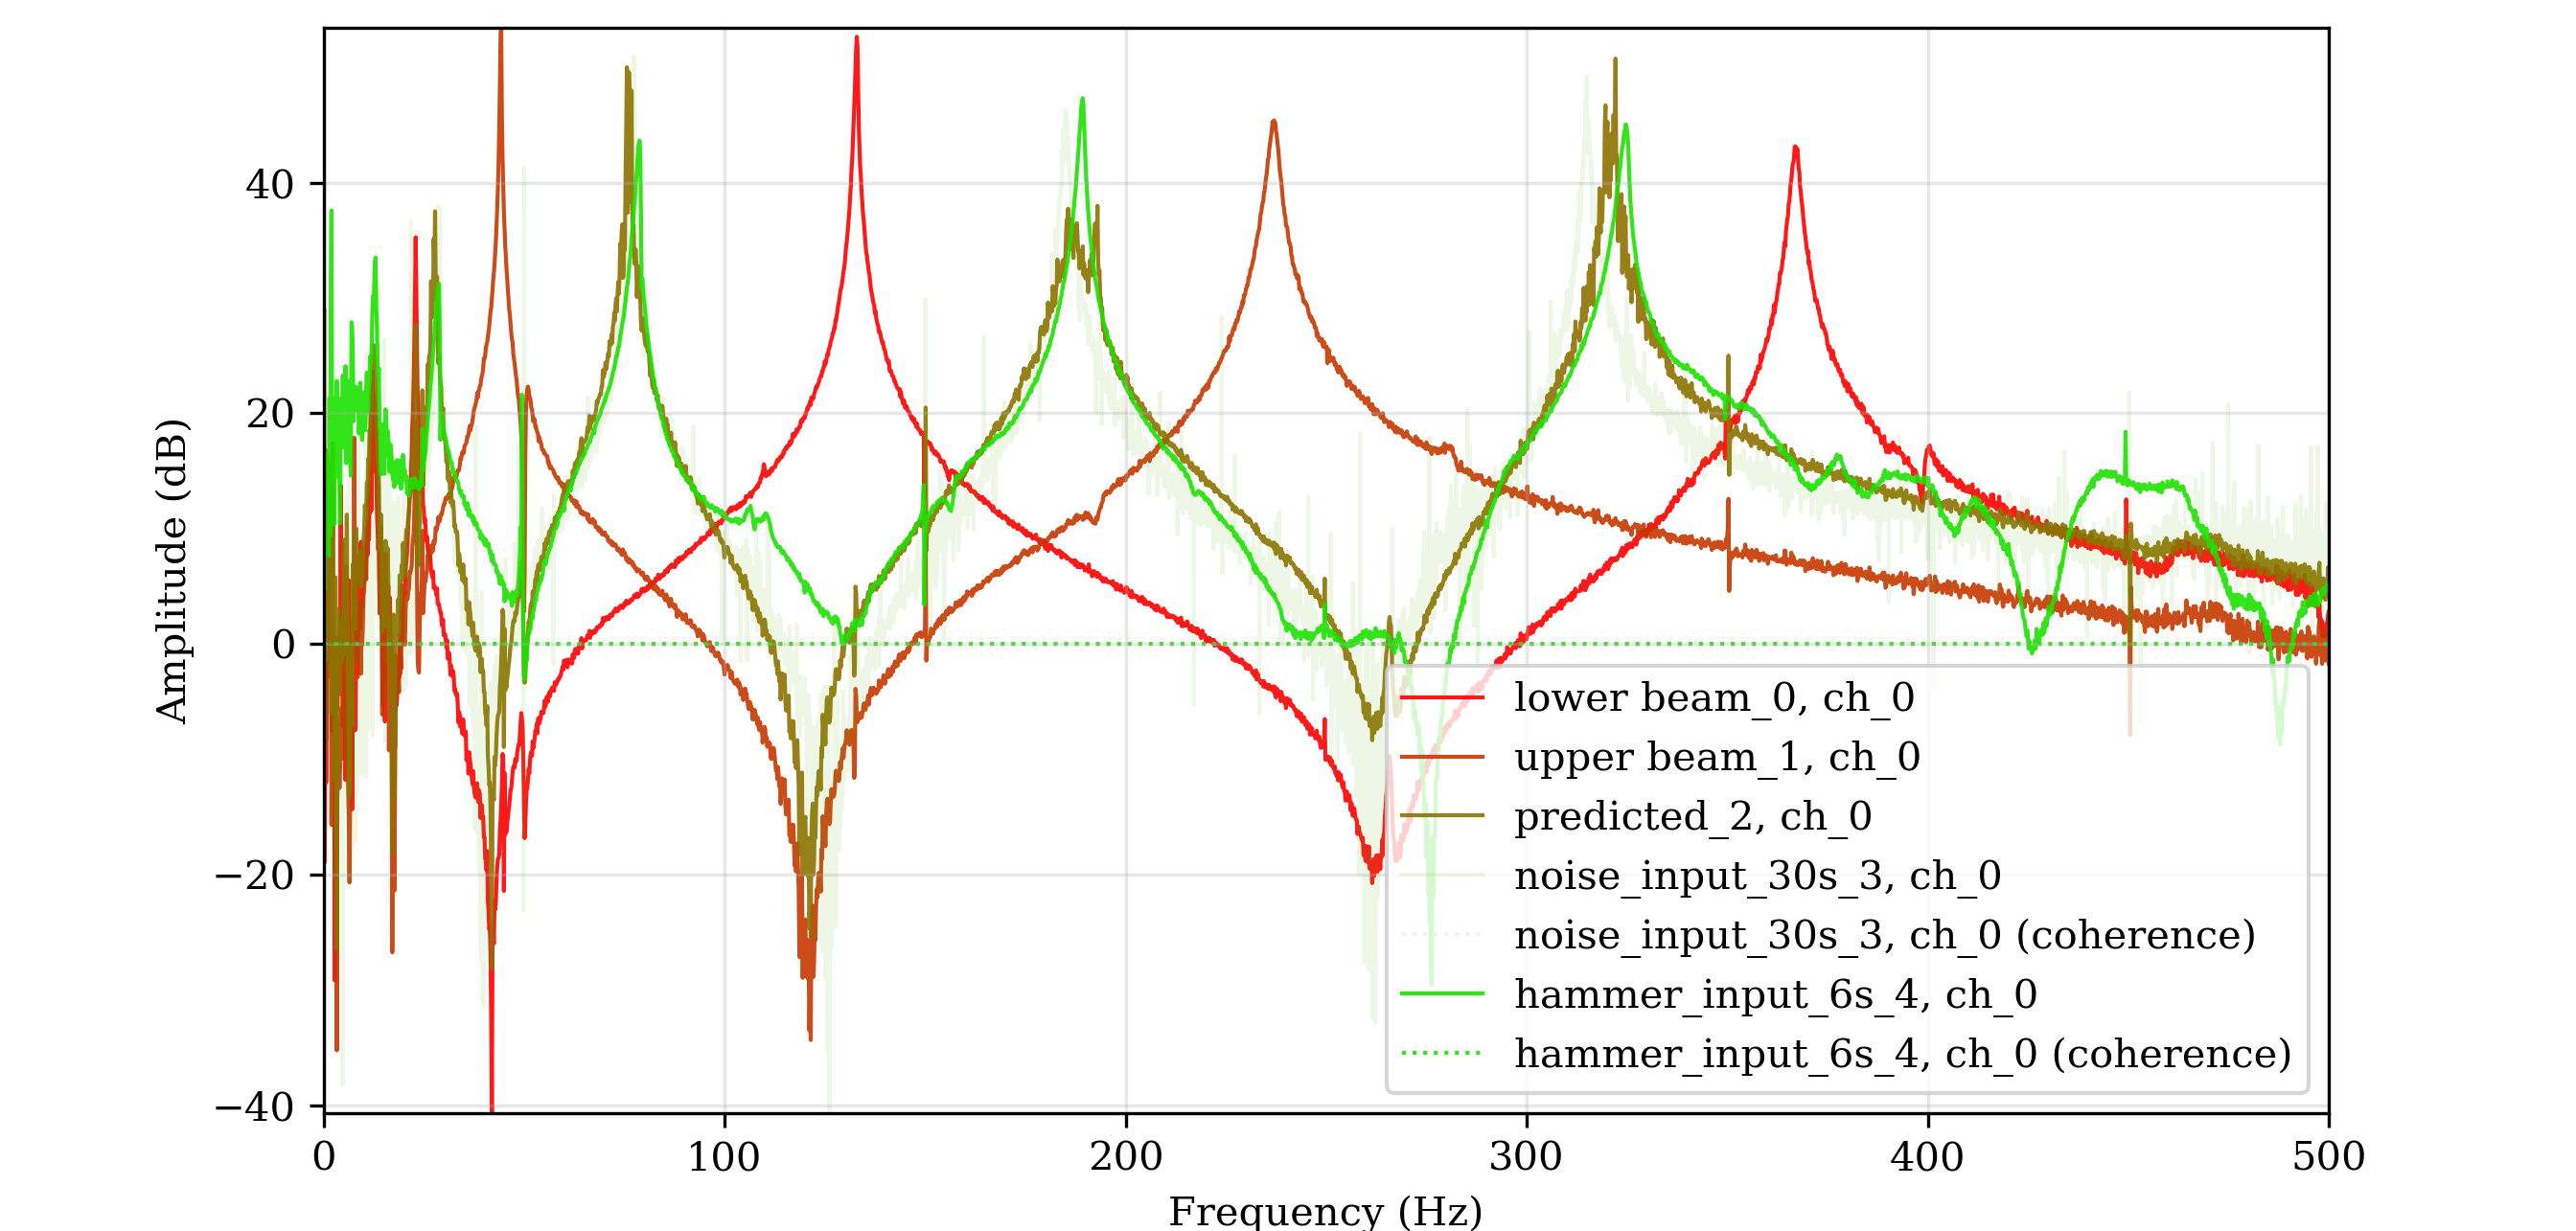
\includegraphics[width=\linewidth]{6-coupledcomp}
  \caption{Transfer functions of the predicted coupled response compared to the response when a hammer is applied to the coupled system }
  \label{fig:coupledcomp}
\end{figure}
\begin{equation}
\label{coupledeq}
\begin{split}
&\frac{1}{Y_{coupled}(\omega )}= \frac{1}{Y_{top}(\omega )} + \frac{1}{Y_{bot}(\omega )}\\
&Y_{coupled}(\omega) = (\frac{1}{Y_{top}(\omega )} + \frac{1}{Y_{bot}(\omega )})^{-1}   = \frac{Y_{top} Y_{bot}}{Y_{top}+Y_{bot}} \\
\end{split}
\end{equation}


Figure \ref{fig:coupledcomp} shows the predicted coupled behaviour compared to the hammer excitation on the coupled system. The resonant peaks agree closely with more noise present in the predicted curve. However, anti-resonances appear smoother and at lower frequencies in the predicted response. The resonant peaks also appear at a marginally lower frequency in the predicted response. This is due to the mass of the accelerometer and magnet being counted twice due to two measurements, this additional mass is greater than the coupling bar which has been removed. Therefore, the prediction is for a higher mass and $\omega \propto \sqrt{\frac{k}{m}}$ therefore a lower frequency is expected. 
\newline
In order to remove discrepancies between measured and predicted responses the following could be implemented:
\begin{itemize}
\item Ensure the connection rod is made of a rigid material with low damping. This helps enforce the boundary condition in coupling where both parts have the same velocity. This could be done through screw in connections, however this would decrease the ease of changing the structure.
\item Lighter accelerometer or use of a laser vibrometer to minimise the effect of double counting the added mass.
\end{itemize}


\subsection{Transfer Function theory}
The apparatus consists of two coupled cantilever beams, the bending of each beam follows equation \ref{eq:difeq}. With x being the distance from the fixed end, and y the vertical displacement. After the initial impulse free vibration occurs as f(x,t)=0. The structure is exited and measured from 0.155m. At this location a node occurs nearby in the third mode for the upper beam and fourth mode for the lower, these modes would be attenuated in the measurement. However, they occur outside our frequency range therefore smaller resonant peaks shouldn't be observed which agrees with the observation. 

\begin{equation}
\rho A\frac{\partial^2 y}{\partial t^2} + EI \frac{\partial^4y}{\partial x^4} = f(x,t)
\label{eq:difeq}
\end{equation}

The solution to this motion with a fixed boundary condition at x=0 and free condition at x=L satisfies equation \ref{eq:sol}. For n=1 this gives kL=1.8751 and higher modes $k_nL \approx (n-\frac{1}{2})\pi$ or the ratio between $\omega$ of 1 : 6.3 : 17.5 : 34.4. 
For the lower beam the resonant frequencies (ignoring the resonant caused by the rubber feet) follow the pattern 23, 130 and 370Hz this is the ratio: 1: 5.65 : 16.1. Similarly the upper beam follows 44, 237 Hz or the ratio 1 : 5.38. Both of these show that the frequencies agrees to some extent with the theory. However, the pattern is hard to distinguish off so few data points. The measured ratio's are likely to vary as they're highly dependant on the reading for the lowest resonance, small changes to this can massively effect the frequency ratio. These small changes could arise from the low SNR around the lower frequencies. The differing ratios also arise from the additional mass lowering the higher resonant frequencies by more than the first mode see figure \ref{fig:TFtheory}.

\begin{equation}
\begin{split}
& coskLcoshkL=-1\\
& k^2_n = \omega_n\sqrt{\frac{\rho A}{EI}}\\
\end{split}
\label{eq:sol}
\end{equation}

 The lower beam had a length of 48.5cm compared to 33cm therefore its expected to have lower natural frequency's. The ratio between the first natural frequency of the lower beam and upper should be the reciprocal of the length ratio. $\omega_{top}:\omega_{bot} = 1:1.8$, $L_{top}:L_{bot}=1.47:1$ this ratio is slightly off. This mismatch is due to an additional mass located on the upper beam which lowers the resonant frequencies and therefore increases the ratio between the two beams. An estimate without this extra mass would be $\omega_{1top}=45/1.47=30.6Hz$.
Using measured lengths and equation \ref{eq:sol} and $k_nL \approx (n-\frac{1}{2})\pi$ for n>1 or kL=1.8751 for n=1 you get the theoretical resonant frequencies listed in table \ref{table:theoryw}.



\begin{figure}[!htb]
  \centering
    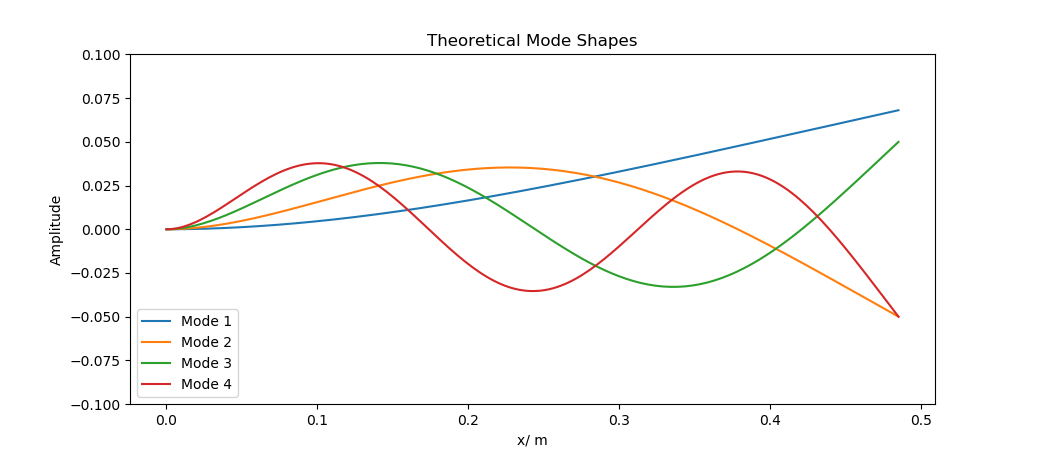
\includegraphics[width=\linewidth]{modeshapes}
  \caption{Theoretical mode shapes for the lower cantilever beam}
  \label{fig:modeshape}
\end{figure}

\begin{table}[h]
\caption{Theoretical natural frequencies with $A_t=A_b=5cmx6mm=3x10^{-4}m^2$, $I_t=I_b=\frac{5cm*(6mm)^3}{12}=9x10^{-10}m^4$, $L_t=0.33m$, $L_b=0.485m$, $\rho \approx 7.8x10^3kg/m^3$ and $E \approx 210x10^9Pa$}
\centering
\begin{tabular}{ c | c | c | c | c }
n & $\omega_{bot}/Hz$ theory & $\omega_{bot}/Hz$ measured &$\omega_{top}/Hz$ theory & $\omega_{top}/Hz$ measured \\

\midrule
1 & 21.4 & 23 & 46.2 & 44 \\
2 & 135.0 & 130 & 291.7 & 237\\
3 & 375.1 & 370 & 810.2 & - \\
\end{tabular}
\label{table:theoryw}
\end{table}

Theoretical transfer functions for admittance can be generated by using the formula given in equation \ref{eq:theoryTF}. The measuring(k) and driving(j) point are both the same and are at 0.155m, $u_j^{(n)}u_k^{(n)}$ are the mass normalised mode shapes. The damping ratio $\zeta$ was chosen to be 0.005 during calculations. The standard transfer function is multiplied by $i\omega$ to relate it to velocity instead of position. Theoretical mode shapes before normalisation can be seen in figure \ref{fig:modeshape} and various transfer functions in figure \ref{fig:TFtheory}. Code for generating these graphs can be seen in the appendix section 1.  

\begin{equation}
\mathcal{G}(j,k,\omega)= \frac {\dot{Y}}{F}=\sum^\infty_{n=1} \frac{u_j^{(n)}u_k^{(n)}}{\omega_n^2-\omega^2 +2i\zeta \omega_n \omega} i\omega
\label{eq:theoryTF}
\end{equation}

\begin{figure}[!htb]
  \centering
    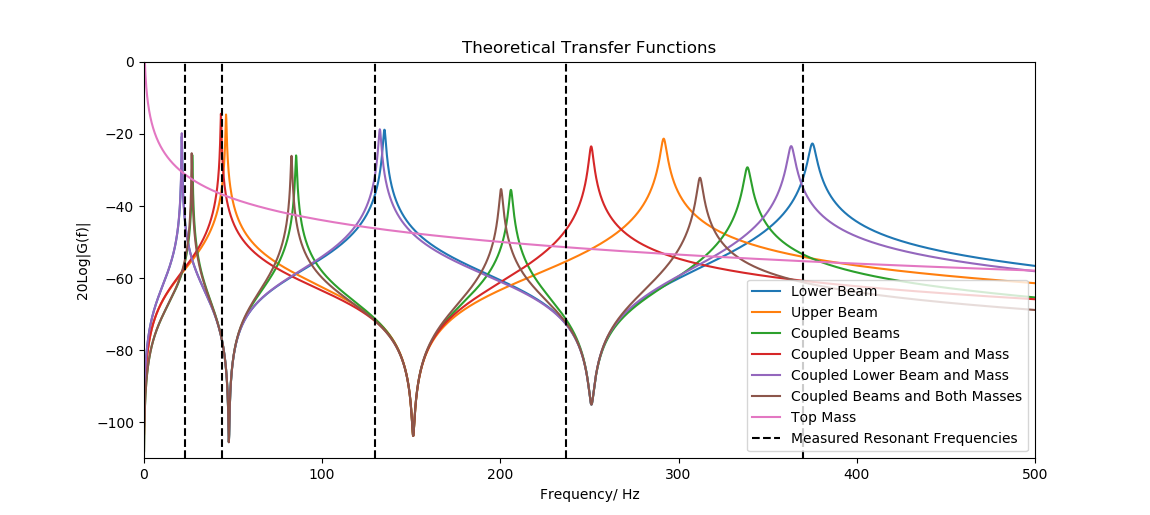
\includegraphics[width=\linewidth]{TFtheory}
  \caption{Theoretical transfer functions for different situations of coupling}
  \label{fig:TFtheory}
\end{figure}


The transfer function between velocity and force for a mass is $\mathcal{G}(\omega)=-\frac{i}{\omega m}$, this was calculated for a mass of 0.21kg for the extra block and 0.04kg for the accelerometer. Figure \ref{fig:TFtheory} shows that adding an additional mass to the upper beam greatly improves the accuracy of the second resonant frequency. Strangely on the lower beam the highest resonant frequency was predicted lower than what was measured when the mass was considered, even though the other resonant peaks are all predicted at higher then measured values. Comparing these predictions to the calibrated response in figure \ref{fig:3a} its seen that the resonances and anti-resonances both occur in the same range of -20dB to -100dB. this shows that 0.005 is a sensible damping factor as damping determines resonance magnitude.
\subsection{Method comparison}
Table \ref{table:comp} discusses the advantages and disadvantages of each method of force input. A sine sweep is being considered instead of the method we choose as the principal is the same but a sine sweep automates the process across the desired range. This removes the disadvantage of many slow measurements and difficulty in finding resonant peaks. Typical uses for each method is listed in table \ref{table:uses}.


\begin{table}[!htb]
\caption{Comparison of methods of force input}
\centering
\begin{tabular}{ p{46mm} | p{46mm} | p{46mm} }
Sine Sweep & Generated Noise & Hammer Impulse \\
\midrule
\multicolumn{3}{c}{Advantages}\\
Fast to sweep through all frequencies. & Very Fast & Can be calibrated to obtain true velocities and forces.  \\
Fourier transform will have constant magnitude across frequencies of interest, often of a higher magnitude that other methods as each frequency is generated in turn.&The noise can have many forms eg white where each frequency has equal intensity or pink noise where each octave has equal intensity, this makes it very versatile. & Shaker attachment is not required therefore various measurement points can be taken easily and transfer functions throughout the structure can be measured.\\
Guaranteed to include all frequencies of interest. &  Very simply signal to generate. & Less mass added to structure due to lack of a shaker. \\
High SNR therefore is accurate at each measured frequency.& Multiple sample periods can easily be measured and averaged together to create a smooth transfer function with good coherence.& Hammers with greater mass can easily be used in order to provide a larger force to excite more modes. \\
 &A large range of frequencies can be easily generated.& Can work at high temperatures up to 1750$^{\circ}C$ or in vacuums.\\
\midrule
\multicolumn{3}{c}{Disadvantages}\\
Shaker adds mass to structure which lowers resonant frequencies.&Shaker adds mass to structure which lowers resonant frequencies.& Excitation of modes that relate to the structures support.\\
Shaker requires attachment to structure, making it harder to measure transfer function between various locating in the structure.&Shaker requires attachment to structure, making it harder to measure transfer function between various locating in the structure.&Impulse can exceed the operating range of certain devices eg speakers.\\
If shaker attachment is positioned badly additional torsional modes of vibration can be excited.&If shaker attachment is positioned badly additional torsional modes of vibration can be excited.&The presence of high frequencies is low to due an imperfect pulse.\\
&Causality can become a problem if too many frames are used when averaging.&Lower SNR.\\
&Hanning window required to get a smoother transfer function.& \\
\end{tabular}
\label{table:comp}
\end{table}

\begin{table}[!htb]
\caption{Typical applications for each method}
\centering
\begin{tabular}{ p{46mm} | p{46mm} | p{46mm} }
Sine Sweep & Generated Noise & Hammer Impulse \\
\midrule
 Larger structures or models that require high input energy to excite the modes, also additional shaker mass has less effect on a large structure.& Due to the large range of generated frequencies use in acoustic testing where high bandwidth is required.& Quality control and material property/structure measurement due to non-destructive technique and easy of application.  \\
Audio testing, as you can produce an input that contains all the desired frequencies at the same magnitude.&& Measuring the transfer function between lots of locations of a structure. \\
&& Understanding physical properties of high temperature materials.\\
\end{tabular}
\label{table:uses}
\end{table}

\subsection{Damping}
\begin{figure}[!htb]
  \centering
    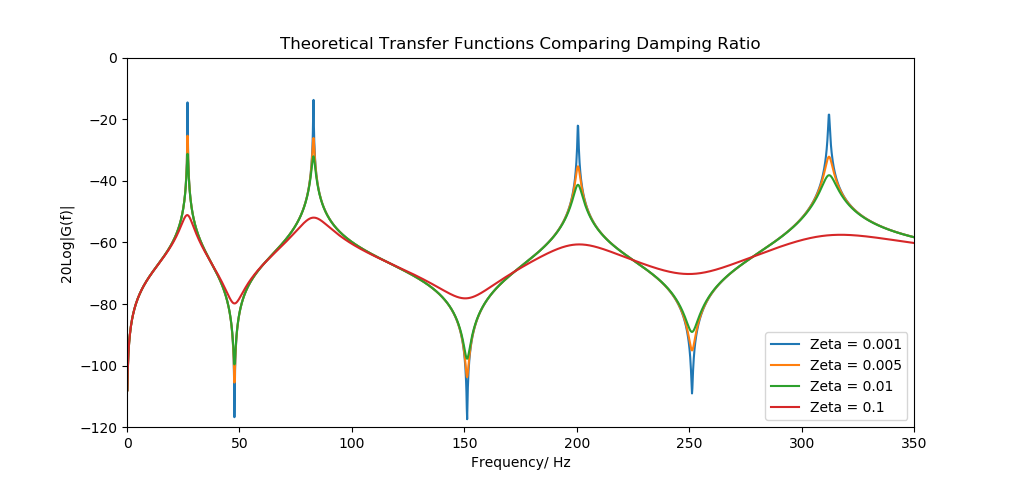
\includegraphics[width=\linewidth]{zetacomp}
  \caption{Theoretical transfer function for the coupled system with various damping ratios}
  \label{fig:zetacomp}
\end{figure}
System damping will reduce the magnitude of resonant peaks and increase the peak width, see figure \ref{fig:zetacomp} for a visualisation of this on the theoretical transfer function of the coupled system. As $\zeta$ increases the validity of the theoretical transfer function decreases as the damping begins to effect the mode shapes and therefore inaccuracies in transfer function are introduced. The frequency of resonance also marginally changes with the addition of damping. From the mechanics data book 4.5 the damped natural frequency is given by equation \ref{eq:dampedfreq}. The damping ratio appears to be approximately $\zeta=0.005$ from comparing peak heights, this means the change is frequency is less than 0.001\% so wouldn't be noticed. The damping factor can be approximated by measuring the half power bandwidth at resonances, $\Delta \omega = 2 \zeta \omega_n$. Measuring on the highest resonance in figure \ref{fig:3a} results in $\zeta \approx \frac{3}{2x340} = 0.0044$, this agrees with the value chosen from peak heights.
Damping ratio is expected to be higher in the coupled system. This is due to additional energy losses occurring in the non perfect connection. The connector rod will flex and dissipate energy, and the ends will move slightly and dissipate further energy. An estimation for uncoupled damping can be made on the highest resonance in figure \ref{fig:uncoupled}, $\zeta \approx \frac{3}{2370} = 0.004$ which is lower than the coupled estimate.
\begin{equation}
\omega_d=\omega_n\sqrt{1-\zeta^2}
\label{eq:dampedfreq}
\end{equation}




%--------------------------------------------------------------

%----------------------------------------------------------------------------------------
\section{Conclusion}
\begin{itemize}
\item Sinusoidal input produces accurate results, but is very time consuming and hard to get defined peaks.
\item Using random noise as the input allows for a very quick method to measure the transfer function. This is provided that the sampling period is long enough to ensure frequencies of interest will be generated.
\item Noise in the transfer function from measuring a noise input can be reduced by splitting up the whole time period into smaller ones and then averaging their transfer functions. Once again this relies on intervals long enough to capture frequencies of interest or coherence will be lost.
\item A hammer can be used as an excitation to approximate an impulse. Due to a finite contact time the high frequencies won't be produced. 
\item Using the hammer allows for an additional resonance peak to be discovered. This relates to the whole structure bending at a lower frequency due to a high mass.
\item Noise in the transfer functions at low frequencies and often anti-resonances occurs as the measured acceleration is low at these points. Therefore sensitivity is also low and measurement noise is prominent. 
\item Decoupling the two beams and measuring individual transfer functions can be used to predict the behaviour of the coupled system accurately. 
\item Damping ratio appears to be 0.005 but is lower in the coupled system due to additional energy losses present.
\item Simulating the transfer function with coupled masses to model additional mass improves the accuracy of the predicted resonances.
\item Each method of force excitation has various advantages and disadvantages that make their use prominent is different areas.
\end{itemize}

\section{Appendix}
\subsection{Theoretical mode shape and transfer function python code}
\begin{lstlisting}
number = 10
n=np.zeros((number,1))
for i in range(number):
    n[i]=i+1
kl=np.zeros((number,1))
kl[0]=1.8751
for i in range(number-1):
    kl[i+1]=(n[i+1]-0.5)*math.pi

L=0.485
L2=0.33
E=210*10**9
p=7800
I=9*10**-10
A=3*10**-4
x=0.155
k=kl/L
k2=kl/L2
zeta=0.005

omegan=k*k*math.sqrt(E*I/(p*A))
omegan2=k2*k2*math.sqrt(E*I/(p*A))
freqarray=np.linspace(1,3500,3500)
Gyf=np.zeros(freqarray.shape,dtype=complex)
Gyft=np.zeros(freqarray.shape,dtype=complex)

D2=0.025
D2t=D2

xs = np.linspace(0,L,200)
for i in range(4):
    D1= -D2 * ((np.cos(k[i]*L)+np.cosh(k[i]*L))
    /(np.sin(k[i]*L)+np.sinh(k[i]*L)))**-1
    ux1 = D1 * np.cos(k[i] * xs) + D2 * np.sin(k[i] * xs) 
    - D1 * np.cosh(k[i] * xs) - D2 * np.sinh(k[i] * xs)
    plt.plot(xs,ux1 , Label = 'Mode ' + str(i+1))

for i in range(number):
    D1 = -D2 * ((np.cos(k[i] * L) + np.cosh(k[i] * L))
     / (np.sin(k[i] * L) + np.sinh(k[i] * L))) ** -1
    ux = D1*np.cos(k[i]*x) + D2*np.sin(k[i]*x) 
    -D1 * np.cosh(k[i]*x) -D2*np.sinh(k[i]*x)
    ux2=ux*ux
    Gyf +=ux2/(omegan[i]**2-freqarray**2 + 2*1j*omegan[i]*freqarray*zeta ) 
    *1j*freqarray

    D1t = -D2t * ((np.cos(k2[i] * L2) + np.cosh(k2[i] * L2))
     / (np.sin(k2[i] * L2) + np.sinh(k2[i] * L2))) ** -1
    ux = D1t * np.cos(k2[i] * x) + D2t * np.sin(k2[i] * x) 
    - D1t * np.cosh(k2[i] * x) - D2t * np.sinh(k2[i] * x)
    ux2 = ux * ux
    Gyft += ux2 / (omegan2[i] ** 2 - freqarray ** 2 + 2 * 1j * omegan2[i] 
    * freqarray * zeta) *1j*freqarray
Gyf = Gyf*10**3  ## for normalisation
Gyft = Gyft*10**3 ## for normalisation
M= 5*10**-2 * 3.6*10**-2 * 1.5*10**-2 *p +0.1
mtf=1/(freqarray**2 *M) *1j*freqarray
\end{lstlisting}


\end{document}
